%%
%% UnBTeX: A class for bachelor, master, and doctoral thesis at the
%% University of Brasilia (UnB), Brazil
%% Version 1.3.2 2023/10/20
%% Copyright (C) 2021-2023 by Henrique C. Ferreira <hcferreira@unb.br>
%%
%% This class file may be distributed and/or modified under the conditions
%% of the LaTeX Project Public License, either version 1.3 of this license
%% or (at your option) any later version. The latest version of this
%% license is in:
%% 
%%    http://www.latex-project.org/lppl.txt
%% 
%% and version 1.3 or later is part of all distributions of LaTeX version
%% 2005/12/01 or later.
%%
%% This file is a template for use with the UnBTex class
%% To compile the document you should call pdflatex, bibtex, pdflatex
%% 

\documentclass[
	% -- opções da classe memoir -- https://www.ctan.org/pkg/memoir
	12pt,				% tamanho da fonte
	openright,			% capítulos começam em página ímpar
	                    % (insere página vazia caso preciso)
	oneside,			% caso queira imprimir em frente e verso, use
	%twoside,
	a4paper,			% tamanho do papel.
	sumario=tradicional,
	% -- opções do pacote babel --
	english,           % o idioma do texto não é definido aqui (mantenha as oções english e brazil)
	brazil             % para trabalhos em inglês, altere o idioma após o comando \begin{document}
	]{unbtex}

% ---
% Pacotes básicos (Adicione abaixo pacotes úteis para o seu trabalho)
% ---

% Bibliografia nas normas da ABNT, formato autor-data
% O formato autor-data facilita a leitura, sobretudo de trabalhos com muitas páginas
\RequirePackage[english,brazilian,hyperpageref]{backref}	 % Paginas com as citações na lista de referências
\RequirePackage[alf,abnt-etal-list=0,abnt-etal-cite=3,bibjustif]{abntex2cite}

% Referências cruzadas automáticas, dependendo do tipo de referência (figuras, tabelas, equações, etc.)
\RequirePackage[nameinlink,noabbrev,english,brazilian]{cleveref}
\usepackage{multicol}

% ---
% Compila o índice
% ---
\makeindex
% ---

% ---
% Compila lista de siglas de siglas e abreviaturas e lista de símbolos
% ---
\RequirePackage[refpage]{nomencl}   % Para gerar lista de siglas e abreviações e lista de símbolos
\newcommand{\makenomencl}{
\makenomenclature
\renewcommand{\nomname}{\listadesiglasname}
\def\pagedeclaration##1{\dotfill\hyperlink{page.##1}{\nobreakspace##1}\par}
\renewcommand{\nomgroup}[1]{%
    % A primeira lista é a de abreviaturas e siglas
    \ifstrequal{##1}{A}{\vspace{-36pt}
    \item[]%
    }{%
    \ifstrequal{##1}{B}{
    % Força a criação de uma nova lista, a lista de símbolos
    \cleardoublepage\chapter*{\hspace{-\leftmargin}\listadesimbolosname}
    % Cria o grupo de símbolos romanos
    \item[{\bfseries\color{verdeunb}\sffamily\large Símbolos romanos}]}{}
    }{%
    \ifstrequal{##1}{C}{\vspace{20pt}
    % Cria o grupo de símbolos gregos
    \item[{\bfseries\color{verdeunb}\sffamily\large Símbolos gregos}]
    }{}
    }{%
    \ifstrequal{##1}{D}{\vspace{20pt} \item[{\bfseries\color{verdeunb}\sffamily\large Nome do grupo}]}{}}%
    \hspace*{-\leftmargin}\vspace{12pt}%
} % Os nomes (e quantidade) dos subgrupos da lista de símbolos pode ser customizados
% https://tex.stackexchange.com/questions/257076/customize-vertical-space-of-entries-and-subgroup-names-in-nomenclature
}

% ---
% Compila a nomenclatura
% ---
\makenomencl
% ---

% Diretório das figuras
\graphicspath{{unbtex-example/figuras/}}
% --- 

% ------------------------------------------------------------------------
% ------------------------------------------------------------------------
% Informações do trabalho
% ------------------------------------------------------------------------
% ------------------------------------------------------------------------

% Título (no idioma do texto)
\titulo{Sistema baseado em machine learning \\ para classificação de queimadas ao longo do \\ território brasileiro utilizando dados de satélites} % insira \\ para forçar quebras de linha no título
% Não utilize caixa alta para o título do trabalho e nem das seções (com exceção de siglas)
% Em inglês caso o trabalho seja em inglês.
\tituloestrangeiro{}
% Obrigatório título em português caso o texto do trabalho seja em inglês (caso contrário, deixe vazio)

% Autores
\autori[]{Caio}{de Lima Saigg} % \autori[]{Nome}{Sobrenome}
% No caso de nomes como Carlos de Souza, utilize \autori[]{Carlos de}{Souza} (e não \autori[]{Carlos}{de Souza})
\autorii[]{Ian}{Porto e Mello} % deixe os argumentos vazios se não tiver segundo autor

% Orientadores
\orientador[Prof. Dr.]{Edson}{Mintsu Hung} % É possível alterar o gênero para orientadora mais abaixo, após o comando \begin{document}
\coorientador[Prof. Dr.]{}{} % deixe os argumentos vazios se não tiver coorientador 
% É possível alterar o gênero para coorientadora mais abaixo, após o comando \begin{document}

% Tipo de trabalho
\tipotrabalho{Projeto Final de Curso} % Dissertação de Mestrado; Tese de Doutorado (em português, mesmo que o trabalho seja em inglês)
\tipocurso{Engenharia de Controle e Automação} % Programa de Pós-Graduação em Engenharia Elétrica (em português, mesmo que o trabalho seja em inglês)
\preambulo{Projeto Final de Curso submetido como requisito parcial para obtenção do grau de Engenheiro de Controle e Automação} % Texto que aparece na folha de rosto e na folha de aprovação. Pode variar, por exemplo, de acordo com o tipo de trabalho (Trabalho de Conclusão de Curso, Dissertação de Mestrado, Tese de Doutorado), do grau (Bacharel, mestre, doutor) e do curso. Consulte a secretaria/coordenação do curso para saber o que deve ser escrito no preâmbulo. Use português mesmo que o trabalho seja em inglês.

% Instituição
\instituicao[Universidade de Brasília]{Faculdade de Tecnologia}{}
%\instituicao[Universidade de Brasília]{Faculdade de Tecnologia}{Departamento de Engenharia Elétrica}  % comente a linha acima e retire o comentário desta linha caso queira incluir o departamento da unidade acadêmica
% Use português mesmo que o trabalho seja em inglês.

% Local e data
\local{Brasília}
\dia{29}
\mes{julho}
\ano{2022}

% Palavras-chave (pelo menos três devem ser informadas)
\pchavei{Monitoramento da Amazônia}
\kwordi{Amazon Monitoring}
\pchaveii{Aprendizado de máquina}
\kwordii{Machine Learning}
\pchaveiii{Queimadas}
\kwordiii{Fire} % deixar vazio se não tiver

% Código Cutter para a ficha catalográfica:
% A ficha catalográfica deve conter o código Cutter, que pode ser obtido com a ajuda de alguns sites da internet (por exemplo, https://www.tabelacutter.com/). O sobrenome do primeiro autor é associado a um número com dois ou três dígitos, que deve ser utilizado como argumento do comando \numerocutter presente no arquivo *.tex principal do relatório. No caso de nomes como Carlos de Souza, utilize 'Souza, Carlos de' (e não 'de Souza, Carlos') para gerar o código.
% Quando compilar o arquivo, a ficha catalográfica gerada terá antes e depois do número de dois ou três dígitos, a primeira letra do sobrenome (em maiúsculo) e a primeira letra do título do trabalho (em minúscula), respectivamente.
\numerocutter{769} % Correspondente à entrada: Lisboa, Carlos

% Membros da banca
\membrodabancai{Prof. Dr. Edson Mintsu Hung, UnB/FT/ENE} % Membro 1 - Geralmente é o orientador
\membrodabancaifuncao{Orientador} % Em português mesmo que o trabalho seja em inglês.
\membrodabancaii{Prof. Dr. } % Membro 2
\membrodabancaiifuncao{Examinador interno}
\membrodabancaiii{Prof. Dr. } % Membro 3
\membrodabancaiiifuncao{Examinador interno}
\membrodabancaiv{} % deixar vazio se não tiver o quarto membro
\membrodabancaivfuncao{Examinador externo}
\membrodabancav{} % deixar vazio se não tiver o quarto membro
\membrodabancavfuncao{Examinador externo}
% ---

% ------------------------------------------------------------------------
% ------------------------------------------------------------------------
% Início do documento
% ------------------------------------------------------------------------
% ------------------------------------------------------------------------
\begin{document}

% Alterar para o idioma no qual o trabalho será escrito
\selectlanguage{brazil}
%\selectlanguage{english} % Para trabalhos escritos em inglês, é obrigatório conter um apêndice com resumo estendido em língua portuguesa.

\IfStrEq*{\languagename}{brazil}{
\thmnamebr
\renewcommand{\bibname}{Referências}
\renewcommand{\lstlistingname}{Código}
\renewcommand{\orientadorname}{Orientador} % O gênero pode ser alterado para Orientadora
\renewcommand{\coorientadorname}{Coorientador} % O gênero pode ser alterado para Coorientadora
\renewcommand{\anexoname}{Anexo}
\renewcommand{\apendicename}{Apêndice}
}{
\thmnameen
\renewcommand{\bibname}{References}
\renewcommand{\lstlistingname}{Code}
\renewcommand{\orientadorname}{Orientador} % O gênero pode ser alterado para Orientadora. Não alterar para Supervisor/Advisor, mesmo que o trabalho seja em inglês.
\renewcommand{\coorientadorname}{Coorientador} % O gênero pode ser alterado para Coorientadora. Não alterar para Co-Supervisor/Co-Advisor, mesmo que o trabalho seja em inglês.
\renewcommand{\anexoname}{Annex}
\renewcommand{\apendicename}{Appendix}
}

% Configurações do pacote backref
% Usado sem a opção hyperpageref de backref

\IfStrEq*{\languagename}{brazil}{
\renewcommand{\backrefpagesname}{Citado na(s) página(s):~}
% Texto padrão antes do número das páginas
\renewcommand{\backref}{}
% Define os textos da citação
\renewcommand*{\backrefalt}[4]{
	\ifcase #1 %
		Nenhuma citação no texto.%
	\or
		Citado na p. #2.%
	\else
		Citado nas pp. #2.%
	\fi}%
 }{
\renewcommand*{\backrefalt}[4]{%
    \ifcase #1 %
        No citations.%
    \or
        Cit. on p. #2.%
    \else
        Cit. on pp. #2.%
    \fi}
}
% ---

% ------------------------------------------------------------------------
% ELEMENTOS PRÉ-TEXTUAIS
% ------------------------------------------------------------------------
\pretextual
% ------------------------------------------------------------------------

% ---
% Insere capa
% ---
\imprimircapa
% ---

% ---
% Insere folha de rosto
% ---
\imprimirfolhaderosto*
% ---

% ---
% Insere ficha bibliográfica
% ---
\fichacatalografica
% ---

% ---
% Insere folha de aprovação
% ---
\imprimirfolhadeaprovacao
% ---

% ---
% Insere dedicatória (elemento opcional)
% ---
\begin{dedicatoria}
   \centering
   \vspace*{\fill}
   
   % Primeiro autor
   \textit{Este trabalho é dedicado às crianças adultas que,\\
   quando pequenas, sonharam em se tornar cientistas.} \\
   
   \ifthenelse{\equal{\autoriinome}{}}{}{
   \vspace{1cm}
   \autorinome\ \autorisobrenome \\
   \vspace*{\fill}
   
   % Segundo autor
    \textit{Dedicatória do segundo autor.} \\
   
   \vspace{1cm}
   \autoriinome\ \autoriisobrenome
   }
   \vspace*{\fill}
\end{dedicatoria}
% ---

% ---
% Insere agradecimentos (elemento opcional)
% ---
\begin{agradecimentos}

% Primeiro autor
Agradecemos ao Dr. Lauro César Araujo e equipe que desenvolveram a classe \abnTeX, que pôde ser facilmente customizada para escrita de trabalhos acadêmicos na Universidade de Brasília que atendessem não só as normas da ABNT, como também regras e necessidades específicas de cursos de graduação e pós-graduação.

Agradecemos também ao Prof. Dr. Leonardo Luiz e Castro pelo modelo em \LaTeX\ para livro para editora UnB, com diversas customizações que foram adaptadas para o UnB\TeX.
% ---

\ifthenelse{\equal{\autoriinome}{}}{}{
\vspace{1cm}
\hfill \autorinome\ \autorisobrenome
\vspace{1cm}

% Segundo autor
Agradecimentos do segundo autor.
% ---

\vspace{1cm}
\hfill \autoriinome\ \autoriisobrenome
}

\end{agradecimentos}
% ---

% ---
% Insere epígrafe (elemento opcional)
% ---
\begin{epigrafe}
    \vspace*{\fill}
	\begin{flushright}
		\textit{``If you find that you're spending almost all your time on theory,\\ start turning some attention to practical things; \\ it will improve your theories.\\ If you find that you're spending almost all your time on practice, \\ start turning some attention to theoretical things; \\ it will improve your practice.''\\
		(Donald Knuth)}
	\end{flushright}
\end{epigrafe}
% ---

% ---
% Insere resumos
% ---

% Resumo em português
\newcommand{\imprimirresumo}{
\newpage
\setlength{\absparsep}{18pt} % ajusta o espaçamento dos parágrafos do resumo
\begin{resumo}[Resumo]
% ---
O trabalho propõe o desenvolvimento de um algoritmo baseado em inteligência artificial para monitoramento de incêndios no território da Amazônia Legal, como ferramenta de auxílio para a tomada de ações de preservação e combate a ações ilegais em tempo real. O uso de aprendizado de máquina foi escolhido por ser um método comprovadamente eficaz em projetos de proteção ambiental, que permite rápido reconhecimento de novos eventos com base em informações históricas. O trabalho foca na classificação de incêndios, e para isso os modelos são treinados com uma base de dados pública que não fornece informações em tempo real, mas possui a classificação para diversas queimadas ocorridas nos últimos anos.
% ---
\vspace{\onelineskip}

\noindent
\textbf{Palavras-chave}: \pchaveinome. \pchaveiinome. \pchaveiiinome. \ifthenelse{\equal{\pchaveivnome}{}}{}{\pchaveivnome.}
\end{resumo}}

% Resumo em inglês
\newcommand{\imprimirabstract}{
\newpage
\setlength{\absparsep}{18pt} % ajusta o espaçamento dos parágrafos do resumo
\begin{resumo}[Abstract]
\begin{otherlanguage*}{english}
% ---
This work proposes the development of an algorithm based on artificial intelligence for monitoring forest fires in the territory of the Legal Amazon, as an aid tool for taking preservation actions and combating illegal actions in real time. The use of machine learning was chosen for being a proven effective method in environmental protection projects, which allows fast recognition of new events based on historical information. The work focuses on the classification of fires, and for this the models are trained with a public database that does not provide real-time information, but has the classification for several fires that occurred in recent years.
% ---
\vspace{\onelineskip}
 
\noindent 
\textbf{Keywords}: \kwordinome. \kwordiinome. \kwordiiinome. \ifthenelse{\equal{\kwordivnome}{}}{}{\kwordivnome.}
\end{otherlanguage*}
\end{resumo}}
% ---

\IfStrEq*{\languagename}{english}{
\imprimirabstract
\imprimirresumo}{
\imprimirresumo
\imprimirabstract}

% ---
% Insere lista de ilustrações
% ---
\pdfbookmark[0]{\listfigurename}{lof}
\listoffigures*
\cleardoublepage
% ---

% ---
% Insere lista de tabelas
% ---
\pdfbookmark[0]{\listtablename}{lot}
\listoftables*
\cleardoublepage
% ---

% ---
% Insere as listas de abreviaturas e siglas e de símbolos
% ---
%{\SingleSpacing
\setlength{\nomitemsep}{-\parsep}
\printnomenclature[1.2cm]
% A opção do comando \printnomenclature define a largura da primeira coluna das listas
\cleardoublepage
% ---

% ---
% Insere o sumário
% ---
\pdfbookmark[0]{\contentsname}{toc}
\tableofcontents*
\cleardoublepage
% ---

% ------------------------------------------------------------------------
% ELEMENTOS TEXTUAIS
% ------------------------------------------------------------------------
\textual
% ------------------------------------------------------------------------

% ---
% Capítulo de introdução
% ---
% ----------------------------------------------------------
\chapter{Introdução}
\label{cap_intr}
% ----------------------------------------------------------
\section{Queimadas e Amazônia}
O Brasil é o país com a maior presença da floresta Amazônica na América, 60\% do total da floresta está dentro do território brasileiro, o que equivale a aproximadamente 5 milhoes de quilômetros quadrados ou 59\% do território nacional \cite{tamanhoIBGE}. Por consequência disto, possuimos uma enorme responsabilidade com ela, existente em diversas formas, como na defesa do território nacional ou na proteção de um enorme patrimônio da humanidade. 

Tal patrimônio vem requerendo cada vez mais atenção nos últimos tempos, de acordo com dados gerados pelo PRODES \cite{novatecnica}, entre agosto de 2021 e julho de 2022 a taxa de desmatamento da Amazônia Legal foi cerca de 11594$km^{2}$. Como podemos ver na figura \ref{fig:prodesgraph}, tal taxa vem acompanhando uma alta nos últimos 10 anos do desmatamento no bioma. O INPE \cite{INPE} estima que, desde 1988, 17\% do bioma já tenha sido desmatado. Tais dados reforçam a necessidade de métodos de monitoramento e controle que reduzam as perdas do meio ambiente.

\begin{figure}[htb]
	\centering
	\begin{minipage}{0.9\linewidth}
		\centering
		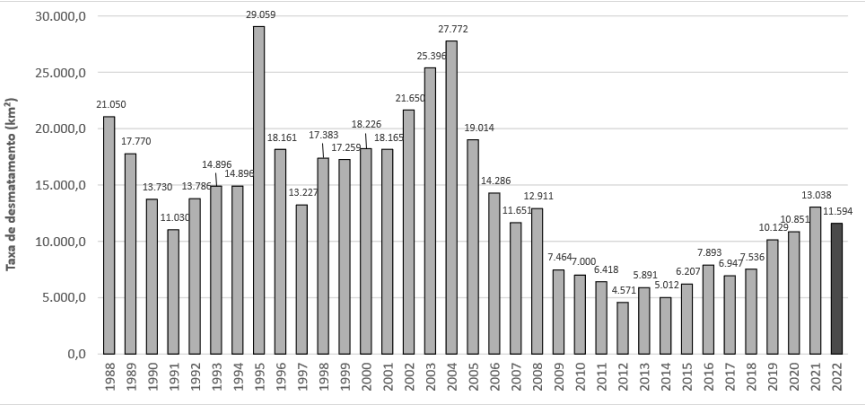
\includegraphics[width=\linewidth]{tg1/figuras/prodes.png}
		\caption{Taxas consolidadas anuais de desmatamento do PRODES \cite{novatecnica}}
            \label{fig:prodesgraph}
	\end{minipage}
\end{figure}

Uma importante área de atuação na preservação da floresta se trata do combate à incêndios. Todos os anos, milhares de quilômetros da floresta amazônicas são queimados por incêndios florestais, causando impactos ecológicos e econômicos, redução da biomassa florestal, mudanças na composição de espécies de árvores e esgotamento do solo \cite{penha}. 

Os incêndios podem ocorrer naturalmente ou podem estar atrelados à atividades humanas. No entanto, queimadas resultantes da ação humana constituem quase que a totalidade dos incêndios registrados nos territórios no Brasil, ocupando o 5º lugar entre os países mais poluidores \cite{bdqueimadas}.

Já as queimadas naturais, por sua vez, costumam ter sua ignição dada por raios, tornando-as mais comuns em períodos de secas prolongadas quando as queimadas costumam atingir seu pico. São mais frequentes no bioma Cerrado que é naturalmente mais seco e adaptado a queimadas naturais recorrentes, normalmente no início e fim das estações chuvosas. Em contraste, o bioma Amazônia é extremamente úmido e apresenta baixos índices de queimadas naturais.

Conforme pesquisas recentes \cite{amazonia_carbono}, a queima e o desflorestamento excessivo na floresta Amazônica está afetando a capacidade de absorção de CO2 da atmosfera, ao mesmo tempo que estas atividades emitem grandes quantidades de carbono por meio da queima de madeira. Além disso, estas ações apresentam um impacto climático na região, tornando a estação seca mais seca, quente e longa, agredindo ainda mais o bioma.

\section{Objetivos}

Os incêndios florestais de origem antropológica são predominantemente e principalmente ligados ao desmatamento e a agricultura de manutenção \cite{severidade}. Nem todo fogo iniciado por atividade humana resultará em tragédia, mas a frouxidão das leis de proteção ambiental estimula pessoas mal intencionadas a queimar grandes áreas públicas para grilagem \cite{jornal_ambiental}, então ser capaz de controlar queimadas é importante tanto para proteger os bens naturais quanto para garantir a aplicação da legislação.

Dessa forma, este projeto visa criar uma ferramenta de \textbf{tipificação automática de incêndios} no território amazônico para auxiliar no combate ao fogo na região. De acordo com o \textit{EU Horizon 2020 Work Programme} \cite{horizon}, o ciclo de gestão do fogo pode ser amplamente segmentado em três etapas: (1) prevenção e preparação (pré-fogo); (2) detecção e resposta (gestão de incêndios florestais ativos); (3) atividades de restauração e adaptação (pós-incêndio). Este trabalho estará focado em desenvolver uma ferramenta que sirva de auxílio para a segunda etapa, na resposta dos órgãos de defesa para com incêndios ativos.

Este trabalho visou o desenvolvimento de um \textbf{algoritmo} projetado para ser incluído ao Painel do Fogo, uma plataforma Web que disponibiliza informações sobre incêndios e queimadas no Brasil, desenvolvido pelo Centro Gestor e Operacional do Sistema de Proteção da Amazônia \cite{painel-fogo}. No entanto, diferente de outras plataformas de monitoramento, o Painel do Fogo trabalha ao lado de batalhões e brigadas no combate ao fogo. Através desta plataforma se é possível obter o 'perímetro' e o “status” mais recente sobre uma queimada ou incêndio de modo que um evento esteja associado a uma ocorrência ou acionamentos de equipes.

O modelo finalizado é capaz de \textbf{classificar queimadas} dentro das quatro classificações utilizadas pelo CENSIPAM para tipificar incêndios florestais na amazônia \cite{andela}: 

%O sistema foi treinado utilizando o extenso banco de dados de queimadas no território Amazônico oferecido pelo Amazon Dashboard do GFED \cite{gfed}. Estes dados são tratados e alimentados a um algoritmo de aprendizado de máquina para o treinamento. O modelo finalizado é capaz de classificar queimadas dentro das quatro classificações utilizadas pelo GFED para tipificar incêndios florestais \cite{andela}: 

\begin{itemize}
    \item  \textbf{Savana e pastagem}: vegetação de porte baixo, com pouca presença de biomassa, longa duração dias-semanas;
    \item \textbf{Pequenas clareiras}: pequenos incêndios em sistemas florestais (cobertura de árvores > 50$\%$ e igual ou inferior a 5 detecções de incêndios), curta duração, área menor que 100 ha;
    \item \textbf{Sub-bosque}: vegetação de porte arbustivo alto, Apresenta altas taxas de biomassa. Ocorre muito em borda de áreas desmatadas com floresta. Área variável, longa duração, poucos focos de calor por detecção, mesma região geográfica do desmatamento;
    \item \textbf{Desmatamento}: os incêndios de desmatamento normalmente têm alto poder radiativo inicial do fogo, pois os detritos lenhosos empilhados levam a uma maior liberação de energia e longa persistência do fogo, uma vez que essas pilhas podem arder por dias. Maior poder radiativo no início, maior duração, área variável.

\end{itemize} 

%Nosso objetivo é gerar nossa própria abordagem de tipificação, embora identificando os mesmos tipos de fogo e usando alguma instância de inteligência artificial, no que couber. No atual estado da arte, o GFED é o único dado a nível mundial com distribuição gratuita na internet que faz referência
%sobre tipos de fogo, mas não disponibiliza queimadas classificadas em tempo real. A diferença na data dos últimos dados disponibilizados para a data real é de cerca de um mês, propomos então um método que possa ser utilizado em tempo real para permitir rápida resposta dos órgãos de proteção ambiental.

A classificação de incêndios florestais desempenha um papel crucial na gestão ambiental, pois fornece informações essenciais para o desenvolvimento de estratégias de prevenção e combate ao fogo. Ao tipificar os incêndios dentro dessas categorias, as autoridades podem avaliar a ameaça que representam para a biodiversidade, comunidades humanas e ecossistemas. Essa análise permite a alocação eficiente de recursos, o planejamento de evacuações quando necessário e a mobilização de equipes de combate a incêndios. Além disso, a classificação de incêndios fornece dados valiosos para estudos e pesquisas que visam entender as causas subjacentes dos incêndios florestais e desenvolver medidas preventivas mais eficazes para proteger as florestas e o meio ambiente.

O Painel do Fogo já possui atualmente capacidade de tipificar seu banco de dados com as quatro classificações de queimada, porém o tempo e pessoal necessário para realizar tão avaliação não permite que estas informações possam ser incluídas na plataforma em tempo real junto com o atual produto da plataforma que é a visualização diária de novos eventos de fogo. O projeto é responsável por realizar tal trabalho de forma ligeira e com um bom nível de acurácia.

Para este fim, a plataforma fará uso de sistemas de \textbf{aprendizado de máquinas} para tipificar queimadas em curso, integrando estas informações à plataforma Web. Através dela, as informações são disponibilizadas para todos que tenham interesse e alertas serão emitidos para os agentes competentes conforme a necessidade.

O uso de inteligência artificial para cuidados durante o ciclo do fogo não são uma novidade, em \cite{invention} foi feita uma revisão de diversos artigos publicados entre 2019 e 2022 que tratavam do uso de métodos de aprendizado de máquina no controle de queimadas florestais. O que se pode concluir da revisão é que existe um potencial para a adoção de métodos de aprendizado de máquina para previsão e classificação e para melhorar o suporte às decisões gerais no monitoramento de danos ambientais relacionados ao fogo.

Em conjunto com um algoritmo de monitoramento, é necessário que acoplado a ele exista um método de fornecimento de dados. A maneira mais comum atualmente de se obter informações do estado mais recente do vasto território da floresta amazônica é por meio do \textbf{sensoriamento remoto}. Compreendendo os tipos de dados que podem ser obtidos por meio do sensoriamento remoto, a relevância deles e sua frequência de obtenção são de grande importância para que uma ferramenta de monitoramento possua um bom êxito.



%\begin{mdframed}[style=defnSty] % azul
%\begin{mdframed}[style=plainSty] % verde

%{\center \textsc{Texto motivador} \par}

%\noindent Esperamos que o \abnTeX\ aprimore a qualidade do trabalho que você produzirá, de modo que o principal esforço seja concentrado no principal: na contribuição científica.
   
%\end{mdframed}
% ---
% ----------------------------------------------------------
\chapter{Trabalhos relacionados}
\label{relacionados}

\section{História do Monitoramento da Amazônia por meio de Sensoreamento Remoto}

Devido ao valor da Amazônia e da necessidade em protegê-la, é natural o interesse em se desenvolver tecnologias de monitoramento visando preservar este grande patrimônio natural. A história do sensoreamento remoto na região data desde o ano 1975, quando foram-se produzidas as primeiras imagens de satélite Landsat, por meio de um sensor MSS ou sensor multi espectral.  Estas imagens compuseram o primeiro grande mapeamento do território para se verificar o potencial desta tecnologia no monitoramento de desflorestamento.

A experiência contemplou uma área de 55 milhões de hectares referentes a uma região crítica ligada a grandes projetos agropecuário, revelando que 10\% do território já estava desflorestado. Diante da indignação internacional oriunda deste conhecimento, as autoridades brasileiras instauraram uma Comissão Parlamentar de Inquérito, ou CPI, para investigar o tema \cite{hist_amz}. 

Em contrapartida, as imagens coletadas para este estudo contemplavam apenas uma parte crítica do território, levantando a dúvida sobre o estado do resto do território. Em 1988, teve origem o projeto PRODES Analógico (Projeto de Monitoramento do Desmatamento na Amazônia Legal por Satélite), produzindo métricas desmatamento anuais para todo o território amazônico até 2003.

\begin{figure}[htb]
	\centering
	\begin{minipage}{0.9\linewidth}
		\centering
		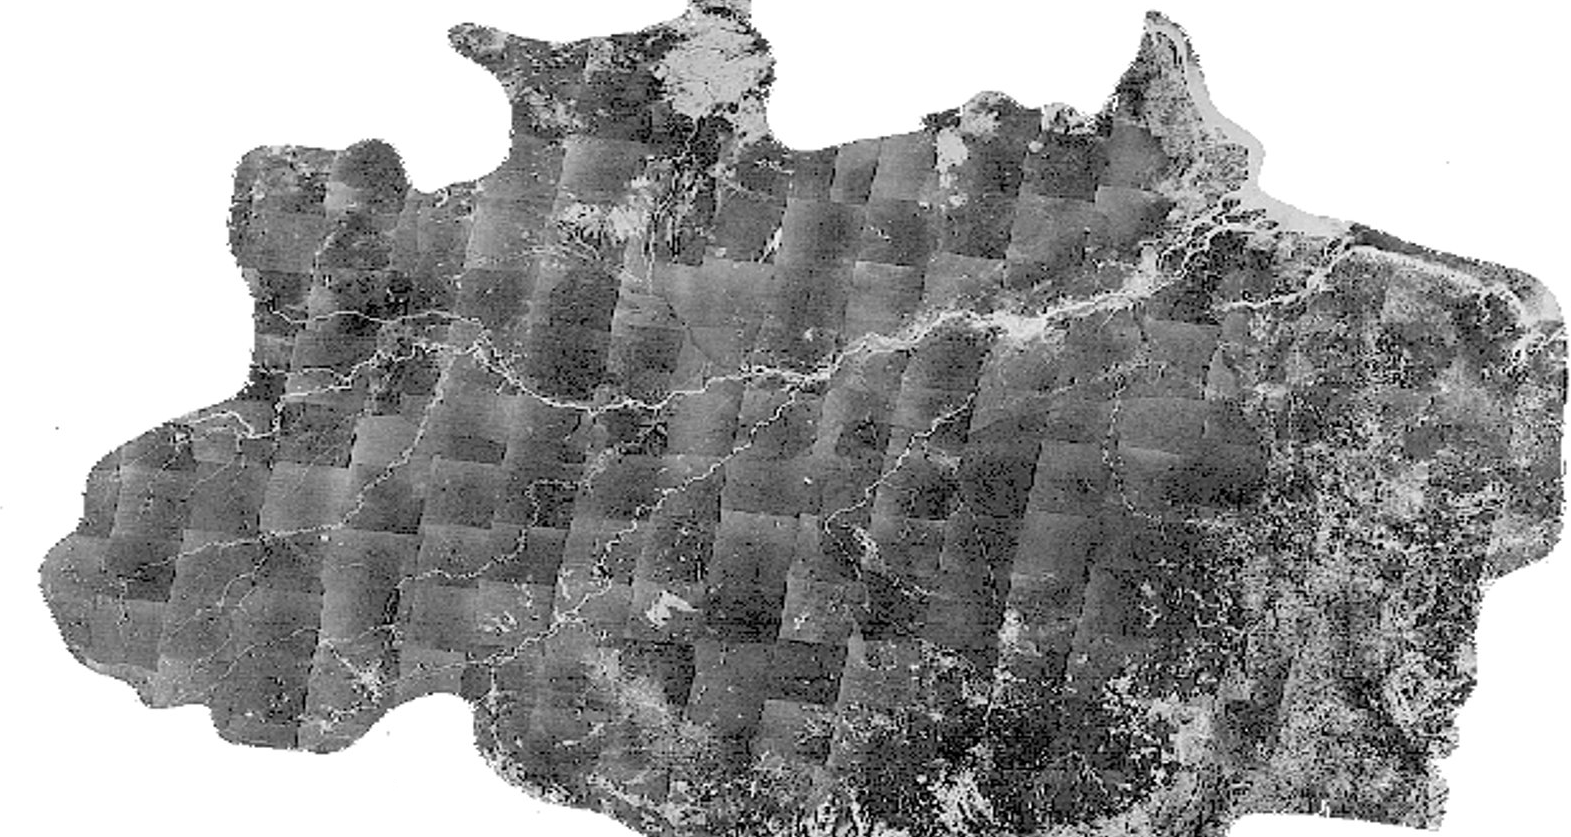
\includegraphics[width=\linewidth]{tg1/figuras/amazon.png}
		\caption{Mosaico com 229 imagens Landsat em escala 1: 250.000 \cite{hist_amz}} \label{fig:amz1988}
	\end{minipage}
\end{figure}

Em sequência, há o nascimento do projeto PANAMAZÔNIA I \cite{panamazonia} em 1992, operando de forma semelhante ao PRODES Analógico. Este novo projeto também faria o monitoramento da amazônia de forma analógica com imagens do satélite Landsat de resolução 1:250.000, visando aumentar a escala e fazer o monitoramento para toda a América do Sul. 

A próxima etapa desta história se da em 1997 por meio do PRODES Digital. Este representou um grande avanço tecnológico na forma da criação de um banco de dados digital, porém, foi limitado a operar dentro da complexidade do projeto PRODES Analógico. Por consequência disto, varias melhorias ao sistema de monitoramento e classificação não foram aplicadas.

A partir de 2003 tem-se a origem do projeto DETER (Detecção do Desmatamento em Tempo Real) \cite{deter}. Esta nova empreitada utilizou imagens do sensor MODIS, abordo do satélite Terra. Apesar da baixa resolução das imagens, tinha-se uma alta taxa de amostragem, gerando-se imagens diárias. A partir disto, o sistema fazia a sobreposição destas imagens e polígonos de desmatamento detectados. Caso um polígono de desmatamento fosse sobreposto a uma imagem de vegetação anteriormente intocada, era gerado um alerta de alteração da cobertura vegetal para os órgãos de fiscalização de desmatamento oficiais. Este foi o primeiro sistema de monitoramento em tempo quase real do território amazônico e opera até hoje.

Em 2020 foi lançado pelo Global Fire Emission Database o \textit{Amazon Dashboard}, uma ferramenta que rastreia incêndios individuais na região da Amazônia usando uma abordagem para agrupar e classificar as detecções ativas em diferentes tipo de incêndio. O GFED é um banco de dados focado em informações de incêndio obtidos por meio de satélites da NASA \cite{gfed}. No atual estado da arte, o GFED é o único dado a nível mundial com distribuição gratuita na internet que faz referência sobre tipos de fogo. 

Em 2021, o Centro Gestor e Operacional do Sistema de Proteção da Amazônia desenvolve o Painel do Fogo, uma plataforma Web que permite visualizar informações em tempo real sobre incêndios florestais na região da Amazônia com o intuito de subsidiar o acionamento de brigadas ou batalhões durante o combate ao fogo. A novidade se baseia em trabalhar agrupamentos de focos de calor para entender se tal situação é um evento individual de incêndio e queimada, e disponibilizá-los no Mapa Interativo de Incêndios e Queimadas.





%No entanto, a floresta Amazônica compreende um território extremamente extenso com uma mata bastante fechada, implicando em um desafio prático e logístico em sua proteção e monitoramento.

%\todo{tem que readaptar muita coisa}


\section{Outros autores na área de monitoramento ambiental}
% ----------------------------------------------------------


Muitos trabalhos abordam a detecção de incêndios florestais, especialmente usando aprendizado de máquina. Vários sensores podem ser usados, como
como câmeras IP \cite{forest-fire-ip-camera}, sensores sem fio para emissão de monóxido de carbono e temperatura \cite{forest-fire-detection-wireless-sensor} e dados de satélite.

\cite{Abid2021} fornece uma visão geral dos sistemas de detecção e previsão de incêndios florestais com base em algoritmos de aprendizado de máquina.
Os estudos que avaliam os fatores que afetam a ocorrência e o risco de incêndio também são discutidos, juntamente com as principais questões e resultados de cada estudo.

Estudos feitos para o bioma Cerrado mostram grande precisão no mapeamento de cicatrizes de queimaduras. O estudo de Arruda \cite{queimadas_cerrado}  teve como objetivo fazer uma metodologia semiautomática para mapeamento de áreas queimadas no Cerrado, utilizando imagens Landsat e algoritmo Deep Learning nas plataformas Google Earth Engine e Google Cloud Storage. O estudo mostrou um potencial de dados de sensoriamento remoto com séries temporais Landsat utilizadas no projeto MapBiomas \cite{MapBiomasQueimadas}.

%\cite{queimadas_cerrado} estava como \cite{UnBVera}


%\todo[inline]{tem dois ARRUDA diferente}


Os estudos para o bioma amazônico são mais escassos. No entanto, Lima \textit{et.al.} \cite{ModisGiovanna} realizou um trabalho focado no mapeamento de cicatrizes de queimaduras na Amazônia a partir de Modelo Linear de Mistura Espectral de imagens de sensores MODIS (MOD09). O estudo foi baseado no DETER (Projeto Detecção de Áreas Desmatadas em Tempo Real) \cite{deter} usando um algoritmo de classificação não supervisionado baseado em regiões. Os resultados mostraram que cerca de 50.000km² da superfície amazônica foram queimados e que os dados diários do sensor MODIS são uma importante fonte de informação para mapeamento de áreas queimadas.

Utilizando dados de sensoriamento remoto, Faria \textit{et.al.} \cite{severidade-do-fogo} desenvolveu um indicador quase em tempo real da severidade do fogo. São usadas informações dos satélites NOAA-20 e Suomi NPP para monitorar eventos de incêndio com base no nível de atenção que eles exigem e em quatro critérios: tamanho geral, duração, extensão e intensidade. A extensão espacial deste indicador inclui os biomas Amazônia e Pantanal brasileiros.

Bruno Scholles \cite{BrunoScholess2023}, em conjunto com os autores e o conteúdo apresentado neste trabalho, desenvolveu um sistema de classificação de incêndios dentro da Amazônia Legal utilizando dados de sensoriamento remoto e um método de aprendizado de máquina conhecido como \textit{Random Forest} para integralização com o Painel do Fogo.


\chapter{Metodologia}
\label{metodologia}

A velocidade e a eficiência na detecção e monitoramento dos incêndios florestais são 
fundamentais para a viabilização do controle do fogo, e para isso é necessário possuir informações confiáveis da localidade e da área da queimada \cite{batista}. Visto a importância da preservação do território amazônico, este projeto se dispõe a desenvolver um sistema capaz de classificar por meio de algoritmos de aprendizado de máquina e de dados de satélites esses incêndios. Compondo um sistema inteligente de monitoramento para todo o território Amazônico.

De acordo com \cite{naqa}, “aprendizado de máquina é um ramo em evolução de algoritmos computacionais que são projetados para emular a inteligência humana aprendendo com o ambiente circundante."  Além disso, “pode melhorar automaticamente através da experiência” \cite{coogan}. Ao escolhermos desenvolver a ferramenta por meio de algoritmos de aprendizado de máquina, temos o objetivo de que ela possa fazer de maneira autônoma um trabalho de monitoramento que até então precisava da supervisão de um ser humano. % como fora feito anteriormente por muitos anos em projetos como o PRODES Analógico.

O trabalho aqui apresentado melhor se enquadra em um modelo de pesquisa experimental, onde diversas técnicas de machine learning, processamento de dados, e engenharia de features foram testadas com o objetivo de comparar a eficiência entre elas e como cada elemento é capaz de influenciar no desempenho do algoritmo.

Neste estudo, dados públicos disponíveis gratuitamente na internet foram utilizados como amostras e features para o treinamento da rede. Os dados são disponibilizados por fontes confiáveis e renomadas, utilizadas mundialmente por pesquisadores e órgãos governamentais, como FIRMS e VIIRS, e classificado de acordo com o próprio CENSIPAM e dados do GFED \textit{Amazon Dashboard}. Para treinamento foram utilizadas amostras e informações referentes ao ano de 2020, porém as fontes dos dados são capazes de liberar novos dados frequentemente de forma que o produto final sempre se mantenha atualizado com os conhecimentos mais recentes, podendo entregar suas previsões em tempo real sem que elas percam relevância com o passar do tempo.

É importante salientar que um diferencial dos dados oferecidos pelo Painel do Fogo é a capacidade de monitorar o que chamam de eventos de fogo, observando a evolução de um incêndio ao longo do tempo através de várias detecções de focos de incêndio em proximidade. Dessarte, se é possível analisar um incêndio florestal como um evento variante no tempo.

\todo{mudar? a gente não quer fiscalizar de fato mas classificar apenas né, não identificar}

Como mencionado anteriormente, a qualidade e significância de cada dado dentro do projeto foi analisada experimentalmente. Normalmente ao trabalhar com machine learning e redes neurais é possível medir o quanto que cada informação está sendo importante para as tomadas de decisões do modelo. Realizando tal analise foi-se capaz de definir quais informações deveríamos priorizar a obtenção, e quais não possuiam impacto, assim como quais modelos de aprendizado de máquina aprezentavam melhor desempenho.

Com os resultados preliminares, a próxima etapa é investir em um modelo promissor e criar um código funcional que seja capaz de receber um banco de dados, povoá-lo com as features necessárias e então retornar a saída de forma que ela possa ser incorporada de volta ao banco de dados com o máximo de independência.

A eficácia final do trabalho foi medida tomando como referência o padrão estabelecido pelo CENSIPAN para tipificação de incêndios. Ele também está responsável pela revisão do produto e averiguação de sua utilidade.
\chapter{Fundamentação Teórica}
\label{fund_teo}
% ----------------------------------------------------------

\section{Python}

Python é uma linguagem de programação de alto nível, orientada a objetos e interpretada \cite{van1995python}. Possui uma presença muito forte nos meios acadêmicos e profissionais devido a sua filosofia de priorizar o esforço do programador sobre o esforço da máquina. Em outras palavras, Python é conhecido por sua fácil leitura, aprendizado e rapidez de desenvolvimento de aplicações, além de possuir código aberto e conexões com os mais diversos módulos e \textit{frameworks}.

A linguagem é talvez a mais utilizada no campo de ciência da informação pois, além dos motivos já mencionados, possui diversos módulos de visualização de dados e que, somados à facilidade de leitura do código, proporciona uma visão clara dos dados, até para os não iniciados. Dessa forma, a linguagem é excelente para o desenvolvimento de aplicações de aprendizado de máquina, graças à facilidade da manipulação e visualização de dados e estatísticas e da alta integração com bibliotecas de desenvolvimento de modelos de inteligência artificial.

\section{Scikit-Learn}

Uma biblioteca para Python muito conhecida na área de ciência de dados e de aprendizado de máquinas \cite{sklearn_api}. O projeto de código aberto vem desenvolvendo algoritmos desde 2010, focando na manipulação e tratamento de dados, assim como no desenvolvimento de algoritmos de aprendizado de máquina \cite{scikit-learn}.

O scikit-learn é uma ferramenta valiosa para cientistas de dados, engenheiros de aprendizado de máquina e pesquisadores que desejam explorar e aplicar técnicas de aprendizado de máquina e mineração de dados em seus projetos. Ele permite que os usuários construam, avaliem e ajustem modelos de \textit{machine learning} de maneira eficaz e eficiente, tornando-o uma escolha popular no campo do processamento de dados e aprendizado de máquina.

% \section{Tensorflow 2.0 \& Keras}
% %\todo{PYTORCH}
% Tensorflow 2.0 é uma plataforma de desenvolvimento de algoritmos de aprendizado de máquina em python. No mercado atual, é utilizado amplamente por grandes empresas devido a sua robustez e flexibilidade.  A plataforma é adequada ao uso por profissionais ou amadores, oferecendo um ecossistema capaz de satisfazer as necessidades de ambos \cite{tensorflow2015-whitepaper}.

% Dentro do ecossistema mencionado, existe o módulo Keras. Esta biblioteca providencia uma interface de alto nível para o desenvolvimento de aplicações de aprendizado de máquina de forma fácil de intuitiva \cite{chollet2015keras}.

\section{PyTorch}

Trata-se de uma biblioteca para programação em Python de código aberto amplamente utilizada para o aprendizado de máquina e desenvolvimento de modelos de aprendizado profundo (\textit{deep learning}) \cite{NEURIPS2019_9015}. Ele foi desenvolvido principalmente pelo \textit{Facebook's AI Research lab} (FAIR) e é conhecido por sua flexibilidade e facilidade de uso, o que o tornou uma escolha popular entre pesquisadores e desenvolvedores de aprendizado profundo.

O PyTorch fornece uma estrutura eficiente para realizar operações com tensores, que são essencialmente matrizes multidimensionais, semelhantes às matrizes NumPy. Ele oferece suporte para operações de álgebra linear e cálculo em GPUs, o que o torna adequado para tarefas de aprendizado profundo que envolvem grandes volumes de dados.

Além disso, devido a sua comunidade grande e ativa e a sua flexibilidade, o PyTorch é uma ferramenta poderosa para produção de programas de aprendizado de máquina para as mais variadas aplicações.

\section{Aprendizado de Máquina}

No âmbito de inteligência artificial (IA), isto é, no desenvolvimento de sistemas que simulem a inteligência humana em máquinas ou computadores, existe o campo do Aprendizado de Máquina. Este campo também se dispõe a simular uma inteligência, porém a partir de um processo de treinamento de um algoritmo com um conjunto de dados de forma que o mesmo possa servir para interpretar novos conjuntos.

Aprendizado de Máquina se trata de uma forma de estatística aplicada com a intenção de aproximar funções muito complexas \cite{GoodBengCour16}. Ou seja, é um campo do conhecimento focado no desenvolvimento de algoritmos que possuem uma alta capacidade de generalização após serem treinados a partir de um conjunto de dados. Algumas aplicações destes algoritmos incluem: classificação de conjuntos de dados, detecção de anomalias e regressão (modelamento matemático e previsão de valores).

O campo do aprendizado de máquina teve origem nas décadas de 50 e 60, a partir do \textit{perceptron}, o primeiro modelo de aprendizado de máquina, modelado à imagem de um neurônio \cite{minsky69perceptrons}. Desde então, esta área da ciência vêm evoluindo e passou por uma série de  inovações significativas que reverberaram pela humanidade. Nesta linha, pode-se citar pontos marcantes em sua evolução como o aprendizado profundo, as redes convolucionais e as redes recorrentes, que baseiam o algoritmo desenvolvido neste trabalho.

Algoritmos de aprendizado são separados entre algoritmos supervisionados e não-supervisionados \cite{bishop1995neural}. Os primeiros se referem aos modelos cujo os dados fornecidos são previamente rotulados, possuem sua classificação ou regressão conhecida e estes dados são computados na função de custo no treinamento. Os segundos não possuem dados rotulados e operam tentando agrupar os dados de forma autônoma, formando grupos ou vizinhanças. Estes algoritmos em questão possuem alguns componentes integrais para seu funcionamento: Modelo, Função de Custo e \textit{Dataset}.

\subsection{\textbf{Modelo}}

O modelo é um termo utilizado para descrever a arquitetura geral de um algoritmo de aprendizado de máquina. Diferentes modelos podem ser vastamente diferentes uns dos outros, tanto na forma como processam os dados quanto em sua finalidade mais apropriada. Diferentes características intrínsecas a cada modelo podem torna-lo melhor ou pior para interpretar certo tipos de dados ou objetivos.

% Citando alguns tipos comuns de modelos de aprendizado de máquina temos o \textit{Muti-Layer Perceptron} (MLP), caracterizado por camadas com vários nós, semelhantes a neurônios, com conexões entre si, semelhantes às sinapses. É o modelo mais comum das tais Redes Neurais, apresentando uma camada de entrada e saída e um número qualquer de camadas invisíveis entre ambas \cite{hastie_09_elements-of.statistical-learning}. 

% \begin{figure}[htb]
% 	\centering
% 	\begin{minipage}{0.45\linewidth}
% 		\centering
% 		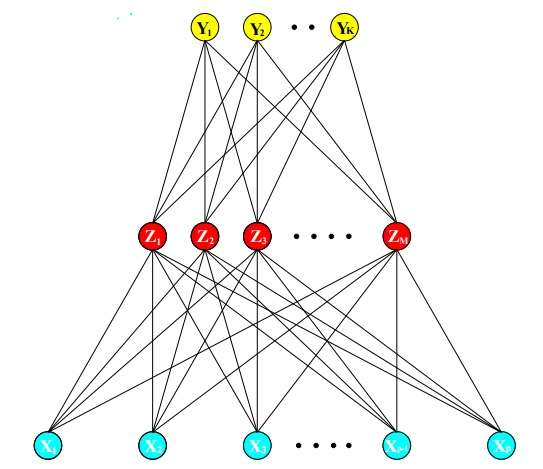
\includegraphics[width=\linewidth]{tg1/figuras/ANN.jpeg}
% 		\caption{Perceptron de Várias Camadas ou MLP \cite{hastie_09_elements-of.statistical-learning}} \label{fig:ANN}
% 	\end{minipage}
% \end{figure}


% \todo{tirar essa parte falando de MLP e RF???}

% Também é frequente utilizar um modelo conhecido como \textit{Random Forest}, um modelo \textit{ensemble}, isto é, um algoritmo que emprega várias cópias do mesmo modelo operando em paralelo. O \textit{Random Forest} produz várias árvores de decisão independentes que processam os dados fornecidos e produzem um resultado final, isto é, cada árvore faz sua classificação ou regressão. A partir disso, o resultado final é decidido por meio de uma "eleição" entre a saída de todas as árvores. Este modelo é bastante empregado para algumas situações por demonstrar bons resultados a partir de dados categóricos, além de ser bem fácil de ser visualizado e interpretado por ser semelhante a uma árvore de cabeça para baixo \cite{oreillyML}

\subsection{\textbf{Função de Custo}}

Todo modelo de aprendizado de máquina faz uso de uma função de custou ou função de erro. Este termo se trata de uma equação que computa a diferença entre a saída do modelo e o resultado esperado, e a partir deste valor os parâmetros do modelo são ajustados de forma a minimizar esta função. 

Utilizando uma linguagem mais matemática, uma estratégia comum de se encontrar um mínimo de uma função se da pelo uso de sua derivada, que fornece o ângulo da curva função em um dado ponto. Ou seja, a partir disto é possível incrementar a função em pequenos valores, encaminhando-a a uma direção onde sua derivada seja nula, isto é, um ponto mínimo. Esta técnica é conhecida como \textit{Gradient Descent} \cite{cauchy}, ou Gradiente Descendente. 



% A situação ideal no treinamento de um modelo é que este atinja um mínimo global, um ponto menor do que todos os outros pontos vizinhos na função de custo. Porém, normalmente se atinge um mínimo local, um ponto que é o menor dentro de sua vizinhança imediata. Isso pode sinalizar o fim do Gradiente Descendente e encerrar o aprendizado em um ponto diferente mínimo global. Em outras palavras, o modelo não minimizou a função da melhor forma possível \cite{GoodBengCour16}.

\subsection{\textbf{Dataset}}
\label{dataset}

O conjunto de dados é vital para o funcionamento do algoritmo de aprendizado. Em geral, o primeiro passo no desenvolvimento de um algoritmo de aprendizado de máquina é a criação de um \textit{Dataset}. Para um modelo tabular, os dados são dispostos na forma de uma tabela enquanto para um modelo convolucional, os dados são fornecidos na forma de imagens. De qualquer forma, uma quantidade suficiente de dados é necessária para um bom treinamento do modelo.

Os dados normalmente são separados em conjuntos de dados de Treinamento e dados de Validação. Dados de treinamento são auto explicativos, isto é, são utilizado para treinar o modelo, enquanto dados de validação são utilizados rotineiramente no treinamento para se checar a acurácia do modelo com um conjunto de dados diferente do utilizado no treinamento. Também é comum de se utilizar um terceiro conjunto, um conjunto de Teste onde o modelo com treinamento concluído processa um novo conjunto diferente para fins de métricas de performance.

%Na internet é possível encontrar vários conjuntos de dados públicos. Um \textit{Dataset} bastante conhecido se chama \textit{MNIST Database} \cite{lecun-mnisthandwrittendigit-2010}, que contém diversas imagens de dígitos manuscritos utilizado para treinar modelos de reconhecimento de escrita por imagens. \todo{é relevante?^^} 
%\todo{falar de serie temporal, redes recorrentes}

\subsubsection{\textbf{Série Temporal}}
Um conjunto de dados de série temporal (ou "dataset" de série temporal) é uma coleção de informações organizadas de maneira sequencial, onde cada ponto de dados está associado a um período de tempo específico. Esse tipo de conjunto de dados é usado para registrar observações, medições ou valores ao longo do tempo. 
Os datasets de séries temporais são frequentemente usados em análises estatísticas, modelagem preditiva e aprendizado de máquina para entender tendências, padrões sazonais e comportamentos ao longo do tempo.

\subsubsection{\textbf{Normalização do \textit{Dataset}}}

Normalizar os dados é uma etapa crucial de pré-processamento que consiste em ajustar as características para uma faixa comum, evitando que valores numericamente mais elevados de algumas características dominem sobre os valores numericamente menores. O principal propósito é reduzir o viés daquelas características cuja contribuição numérica é mais significativa na distinção entre as classes \cite{SINGH2020105524}.

\subsection{\textbf{\textit{Overfitting}}}

\textit{Overfitting}, ou sobreajuste em português, ocorre quando um modelo de machine learning se ajusta excessivamente aos dados de treinamento de maneira que ele passe a falsa impressão de que possui um alto rendimento, porém ao receber dados novos de entrada, a precisão da saída cai consideravelmente \cite{overftt}.

\begin{figure}[htb]
	\centering
	\begin{minipage}{0.9\linewidth}
		\centering
		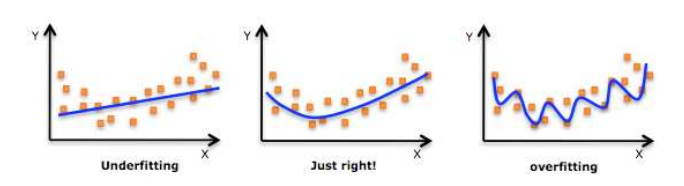
\includegraphics[width=\linewidth]{tg1/figuras/overfiting.png}
		\caption{
            \cite{overftt}} \label{fig:overftt}
	\end{minipage}
\end{figure}

Na imagem \ref{fig:overftt} temos um exemplo de sobreajuste para um modelo de regressão, podemos deduzir do gráfico que a função encontrada é a que melhor minimiza a função de erro do modelo, porém ela certamente não é capaz de ser generalizada para novos dados.

O \textit{overfitting} ocorre quando um modelo é treinado excessivamente nos dados de treinamento, capturando padrões específicos desses dados que não são generalizáveis para novos dados. O modelo acaba por incorporar o ruído dos dados de entrada, levando a previsões imprecisas quando o modelo é exposto a novos dados com ruído diferente.

\subsection{\textbf{Métricas de Avaliação do Modelo}}

A avaliação de modelos de aprendizado de máquina é crucial para desenvolver um bom algoritmo de aprendizado de máquina. Métricas de avaliação fornecem uma medida objetiva do desempenho do modelo, permitindo comparações entre diferentes abordagens.

Métricas são essenciais no ajuste fino dos hiper parâmetros do modelo de aprendizado de máquina. A partir deles, é possível diagnosticar problemas como \textit{overfitting} ou explosão de gradiente. Os dados gerados são acurácia, precisão, \textit{recall} e \textit{f-score} para cada classe e no total de forma ponderada. Além disso também são registrados os valores dos pesos dos nós da rede neural de forma a se observar explosões ou desaparecimentos de gradiente.

\begin{figure}[ht]
    \text{Acurácia} = $\frac{\text{Número de previsões corretas}}{\text{Número total de previsões}}$
    \centering
    \caption{Fórmula para \textbf{acurácia}}
\end{figure}

\begin{figure}[ht]
    \[\text{Precisão} = \frac{tp}{tp+fp}\]
    \centering
    \caption{Fórmula para \textbf{precisão}}
\end{figure}


\begin{figure}[ht]
    \[F_{1} = \frac{2tp}{2tp + fp + fn}\]
    \caption{Fórmula para \textit{F-score}}
\end{figure}

\begin{figure}[ht]
    \[ \textit{recall} =  \frac{tp}{tp + fn}\]
    \caption{Fórmula para \textit{recall}}
\end{figure}

Onde "tp" é quantidade de verdadeiros positivos, "fp" falsos positivos e "fn" falsos negativos. \textit{F-score} é uma métrica útil para medir o aprendizado da rede pois é uma forma de levar em consideração o desequilíbrio entre classes. Por exemplo, em uma tarefa de classificação cujo a classe 1 representa apenas 1\% dos dados teria uma acurácia de 99\% caso exibisse apenas a classe 0 como resultado, porém o \textit{F-score} traria um resultado péssimo, informando a falha da rede. Já o \textit{recall}, que é utilizado no cálculo do \textit{F-score}, mede a capacidade de um modelo identificar corretamente todos os exemplos positivos em um conjunto de dados.

\section{Modelos de aprendizado de máquina}

\subsection{\textbf{\textit{Random Forest}}}

Um modelo \textit{ensemble}, isto é, um algoritmo que emprega várias cópias do mesmo modelo operando em paralelo. O \textit{Random Forest} produz várias árvores de decisão independentes que processam os dados fornecidos e produzem um resultado final, isto é, cada árvore faz sua classificação ou regressão. A partir disso, o resultado final é decidido por meio de uma "eleição" entre
a saída de todas as árvores. Este modelo é bastante empregado para algumas situações por demonstrar bons resultados a partir de dados categóricos, além de ser bem fácil de ser visualizado e interpretado por ser semelhante a uma árvore de cabeça para baixo \cite{oreillyML}.

Cada árvore de decisão é construída dividindo os dados em nós de decisão com base em características específicas. A seleção das características é feita de forma aleatória, o que impede que uma árvore dependa excessivamente de uma única característica, tornando o modelo mais robusto.

\begin{figure}[htb]
	\centering
	\begin{minipage}{0.9\linewidth}
		\centering
		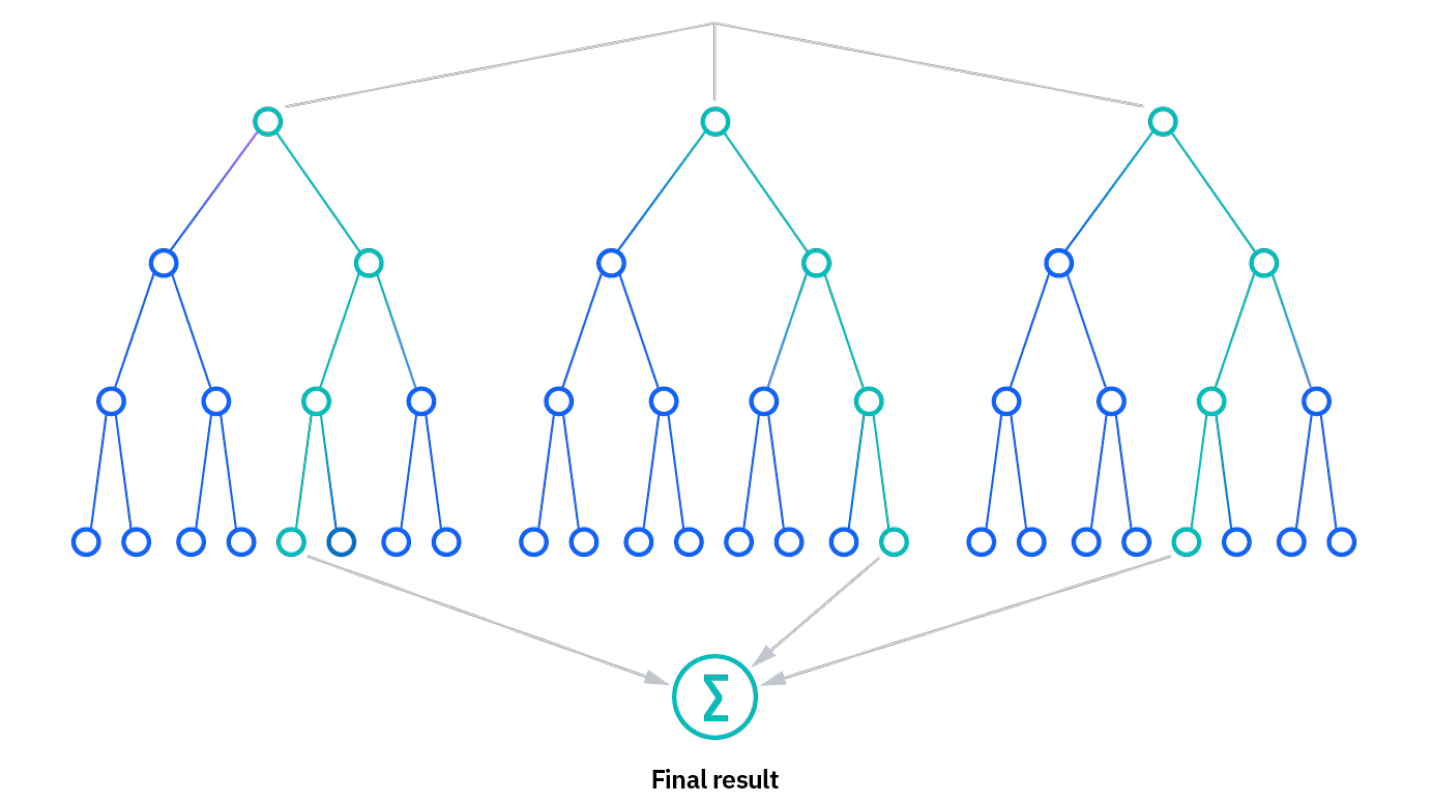
\includegraphics[width=\linewidth]{tg1/figuras/random.png}
		\caption{Ilustração exemplo de um modelo Random Forest
            \cite{rf_fig}} \label{fig:rfmodel}
	\end{minipage}
\end{figure}

\subsection{\textbf{MLP (\textit{MutiLayer Perceptron)}}}

Caracterizado por camadas com vários nós, semelhantes a neurônios,
com conexões entre si, semelhantes às sinapses. É o modelo mais comum das tais Redes Neurais, apresentando uma camada de entrada (Input Layer) e saída (Output Layer) e um número qualquer de camadas invisíveis (Hidden Layer) entre ambas \cite{hastie_09_elements-of.statistical-learning}.

Cada "neurônio" do MLP processa uma combinação linear das saídas da camada anterior por meio de pesos (Weights), aplica uma função de ativação não linear (Activation Function), e passa o resultado para os neurônios na próxima camada.

\begin{figure}[H]
	\centering
	\begin{minipage}{0.9\linewidth}
		\centering
		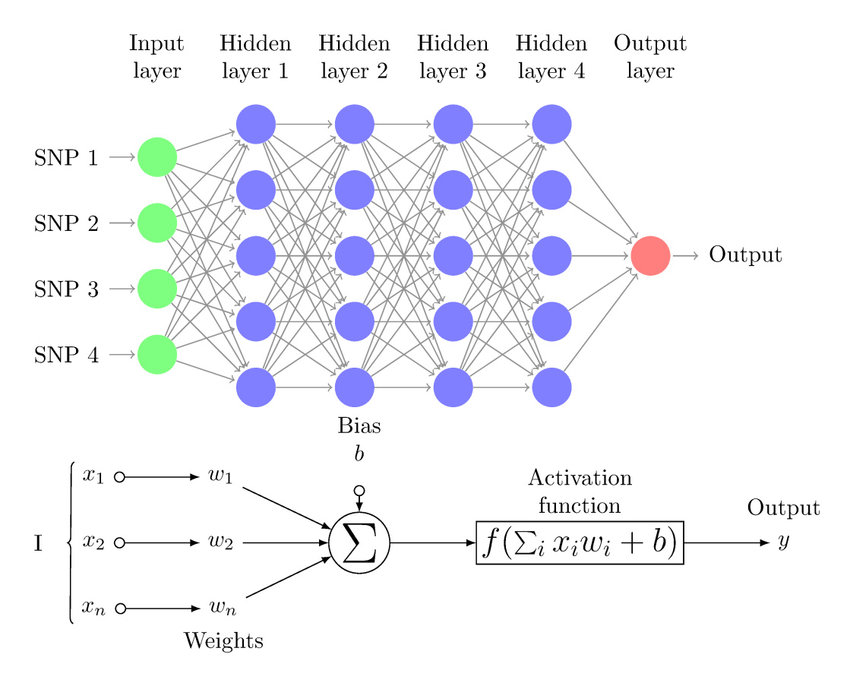
\includegraphics[width=\linewidth]{tg1/figuras/Multi-Layer-Perceptron-MLP-diagram-with-four-hidden-layers-and-a-collection-of-single.png}
		\caption{Ilustração exemplo de um modelo MLP
            \cite{mlp_fig}} \label{fig:mlpmodel}
	\end{minipage}
\end{figure}

\subsection{\textbf{LSTM (\textit{Long Short-Term Memory) }}}

LSTM (\textit{Long Short-Term Memory}) é um tipo de arquitetura de rede neural recorrente (RNN) que é projetada para lidar com sequências de dados e é especialmente eficaz em capturar dependências de longo prazo em sequências temporais \cite{lstm-}. Sua característica fundamental é a capacidade de "lembrar" informações importantes de longo prazo enquanto processam sequências de dados. Isso é alcançado por meio de unidades de memória especiais chamadas células de memória.

\begin{itemize}
    \item Porta de Esquecimento (Forget Gate): Esta porta decide quais informações da célula de memória anterior devem ser esquecidas ou mantidas com base no conteúdo atual da sequência. Ela ajuda a lidar com a questão do esquecimento de informações em sequências longas.
    
    \item Porta de Entrada (Input Gate): A porta de entrada permite que novas informações sejam adicionadas à célula de memória com base na sequência atual. Ela decide quais informações são relevantes para adicionar.
    
    \item Porta de Saída (Output Gate): A porta de saída determina qual parte da célula de memória será a saída da LSTM com base no conteúdo atual da sequência.
    
\end{itemize}

Em questões práticas, a rede neural LSTM recebe três entradas: \textit{cell state} ou estado de célula, \textit{hidden state} ou estado oculto e os dados de entrada. A entrada \textit{cell state} é projetada para capturar dependências de longo prazo em sequências, armazenando e transportando informações relevantes ao longo do tempo e é alterada pelas três portas da rede. Já a \textit{hidden state} é uma representação resumida das informações e pode ser usado como saída da LSTM ou alimentado às camadas subsequentes.

Esta arquitetura de rede neural foi projetada para lidar problemas comuns em redes recorrentes, a explosão ou o desaparecimento do gradiente, a partir do uso das portas e células de memória. Trata-se de uma rede com a capacidade de separar informações irrelevantes, permitindo com que o gradiente não varie caso não seja necessário.

\begin{figure}[htb]
	\centering
	\begin{minipage}{0.7\linewidth}
		\centering
		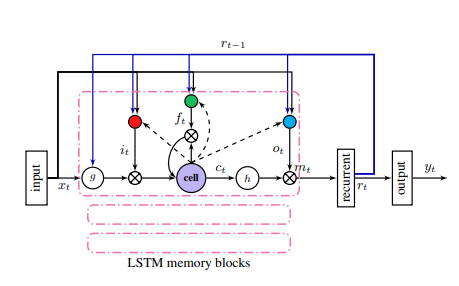
\includegraphics[width=\linewidth]{tg1/figuras/lstm.png}
		\caption{Ilustração exemplo de uma célula de um modelo LSTM
            \cite{lstm_fig}} \label{fig:lstmcell}
	\end{minipage}
\end{figure}

\begin{figure}[htb]
	\centering
	\begin{minipage}{0.6\linewidth}
		\centering
		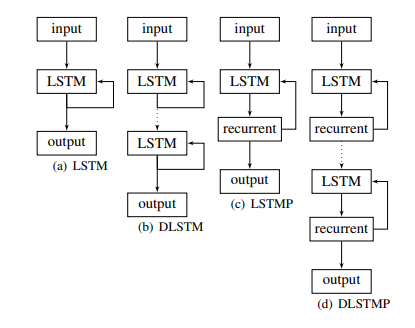
\includegraphics[width=\linewidth]{tg1/figuras/lstm_arch.png}
		\caption{Possíveis arquiteturas com LSTM
            \cite{lstm_fig}} \label{fig:lstmarch}
	\end{minipage}
\end{figure}

\todo{procurar imagens diferentes}



\section{Evento de Fogo}

Os Eventos de Fogo podem ser acessados por meio do Painel do Fogo \cite{painel-fogo}, uma plataforma gerida pelo Censipam \cite{censipam}. Este órgão é subordinado ao ministério da defesa e é responsável por articular ações de governo em prol da proteção ambiental e do desenvolvimento sustentável da Amazônia Legal e da Amazônia Azul.

Os eventos são gerados a partir de observações dos sensores orbitais VIIRS, por meio dos satélites NOAA-20 e SUOMI NPP, e MODIS, por meio dos satélites Aqua e Terra. Estes sensores detectam fogos ativos, formando uma camada vetorial. Em outras palavras, eventos detectados delimitam uma região e quando esta se intersecta com outra durante a mesma passagem do satélite, é gerado um vetor, polígono, que contém todos os eventos detectados na vizinhança e sua evolução ao longo do tempo.


\section{Tipificação do Fogo}

A tipificação do fogo se trata de uma classificação de um evento de incêndio que leva em consideração de diversas condições e características ambientais de forma a classificar o incêndio floresto na região amazônica entre quatro tipos:

\begin{itemize}
    \item \textbf{Savana e pastagem}:  Em regiões onde a vegetação natural é composta principalmente de savana, cerrado ou pastagens, os incêndios frequentemente ocorrem durante a estação seca devido à combinação de condições climáticas secas e atividade humana, como a queima de pastagens para melhorar o crescimento da grama. Vegetação de porte baixo, com pouca presença de biomassa, longa duração dias-semanas;
    \item \textbf{Pequenas clareiras}: Esse tipo de incêndio ocorre em áreas florestais onde as árvores foram cortadas recentemente, criando clareiras. O objetivo pode ser a remoção de resíduos de madeira ou a preparação do solo para o plantio. Pequenos incêndios em sistemas florestais (cobertura de árvores > 50$\%$ e igual ou inferior a 5 detecções de incêndios), curta duração, área menor que 100 ha;
    \item \textbf{Sub-bosque}: Os incêndios no sub-bosque ocorrem em florestas maduras, onde o fogo queima principalmente sob a copa das árvores, afetando a vegetação e o solo abaixo da copa das árvores. Esses incêndios podem ser causados por raios, atividades humanas ou ser usados como ferramenta de manejo florestal. Vegetação de porte arbustivo alto, Apresenta altas taxas de biomassa. Ocorre muito em borda de áreas desmatadas com floresta. Área variável, longa duração, poucos focos de calor por detecção, mesma região geográfica do desmatamento;
    \item \textbf{Desmatamento}: Esses incêndios ocorrem principalmente devido à atividade humana, como a conversão de áreas florestais em terrenos agrícolas, pastagens ou áreas urbanas. São frequentemente associados ao desmatamento ilegal. Os incêndios de desmatamento normalmente têm alto poder radiativo inicial do fogo, pois os detritos lenhosos empilhados levam a uma maior liberação de energia e longa persistência do fogo, uma vez que essas pilhas podem arder por dias. Maior poder radiativo no início, maior duração, área variável.

\end{itemize} 

Os dados necessários para esta classificação são relativos à vegetação (como biomassa e cobertura) e características do incêndio (como persistência e tamanho) \cite{gfed}.

%\begin{mdframed}[style=defnSty] % azul
%\begin{mdframed}[style=plainSty] % verde

%{\center \textsc{Texto motivador} \par}

%\noindent Esperamos que o \abnTeX\ aprimore a qualidade do trabalho que você produzirá, de modo que o principal esforço seja concentrado no principal: na contribuição científica.
   
%\end{mdframed}
\chapter{Banco de dados}
\label{banco}

%\todo{atualizar features}
%\todo{colocar os algoritmos de criação de feature - TCC do scholles}

Como mencionado na subseção \ref{dataset}, a criação de um banco de dados ou \textit{dataset} é fundamental para o treinamento de um algoritmo de aprendizado de máquina. No conjunto de dados devemos especificar quais são os dados de entrada que o algoritmo irá receber e qual a saída esperada para aquela entrada, a partir disso o programa deve fazer uso da função de custo para ajustar os parâmetros do modelo de forma a conseguir acertar a saída com a maior precisão.

Neste trabalho, o banco de dados está no formato tabular, isto é, as informações estão dispostas em uma tabela. Cada linha da tabela possui um conjunto de \textit{features} (os dados de entrada) e um \textit{label} (o rótulo ou saída desejada). Este tipo de conjunto de dados é chamado de \textit{dataframe}, uma estrutura de dados bidimensional com os dados alinhados de forma tabular em linhas e colunas.

Dois bancos de dados foram construídos para a experimentação com diferentes códigos de \textit{machine learning}, o primeiro construído utilizando dados obtidos e rotulados pelo Amazon Dashboard do GFED, e o segundo com dados obtidos e rotulados pelo CENSIPAM. A partir do treinamento com o banco do GFED, foi possível estipular as \textit{features} mais importantes na hora de realizar a tipificação do fogo e que não poderiam ser deixadas de lado na hora de treinar o modelo para trabalhar com o banco do CENSIPAM.

\section{GFED}

Pelo site do Amazon Dashboard é possível fazer o download de um arquivo \textit{.zip} com diferentes tipos de arquivos que contém um mapa da região da floresta amazônica na América do Sul e os diversos eventos de fogo que aconteceram na região desde 2020.
%\todo[inline]{tira as features tudo né. quais ainda usamos?}
\subsection{\textit{Shapefile}}
\label{sec:shp}

O arquivo obtido é do tipo \textit{shapefile}, um formato de armazenamento de dados de vetor para armazenar a posição, forma e atributos de feições geográficas. Este tipo de arquivo pode ser aberto por meio de \textit{softwares} gratuitos como o QGIS, utilizado para visualização de dados GIS (Sistema de Informação Geográfica), para captura de dados, para análise avançada de GIS e para apresentações na forma de mapas, atlas e relatórios sofisticados \cite{qgis}. Um GIS integra informações descritivas a um mapa, eles incluem imagens, feições e mapas base vinculados a planilhas e tabelas.

Ao abrimos o \textit{shapefile} no QGIS, primeiro nos deparamos com uma imagem das queimadas que foram analisadas pelo GFED na região que contém a floresta amazônica desde 2020 até 31 de maio de 2022, como mostrado na figura \ref{fig:mapashp}. Com o projeto aberto, podemos escolher visualizar a tabela de atributos que acompanha o mapa, que está representada na figura \ref{fig:tabat}. A tabela de atributos contém as feições relativas a cada polígono que compõe a imagem do mapa da América do Sul. Os atributos que fazem parte da tabela são:

\begin{figure}[htb]
	\centering
	\begin{minipage}{0.9\linewidth}
		\centering
		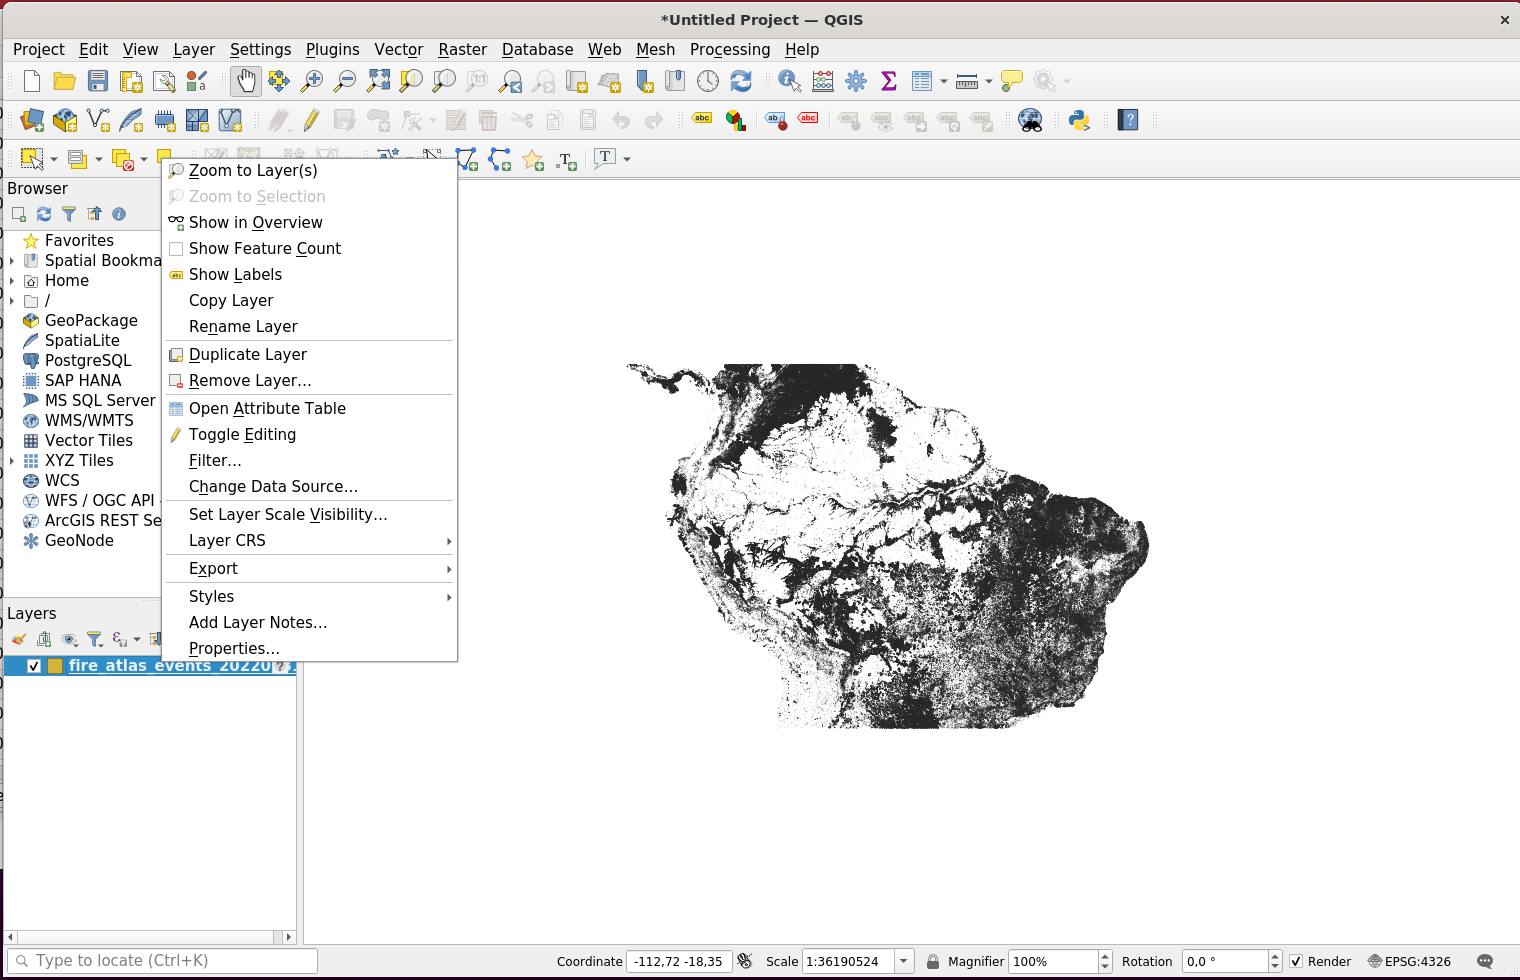
\includegraphics[width=\linewidth]{tg1/figuras/mapa.png}
		\caption{Mapa da América do Sul com os eventos de fogo detectados} \label{fig:mapashp}
	\end{minipage}
\end{figure}

\begin{figure}[htb]
	\centering
	\begin{minipage}{0.9\linewidth}
		\centering
		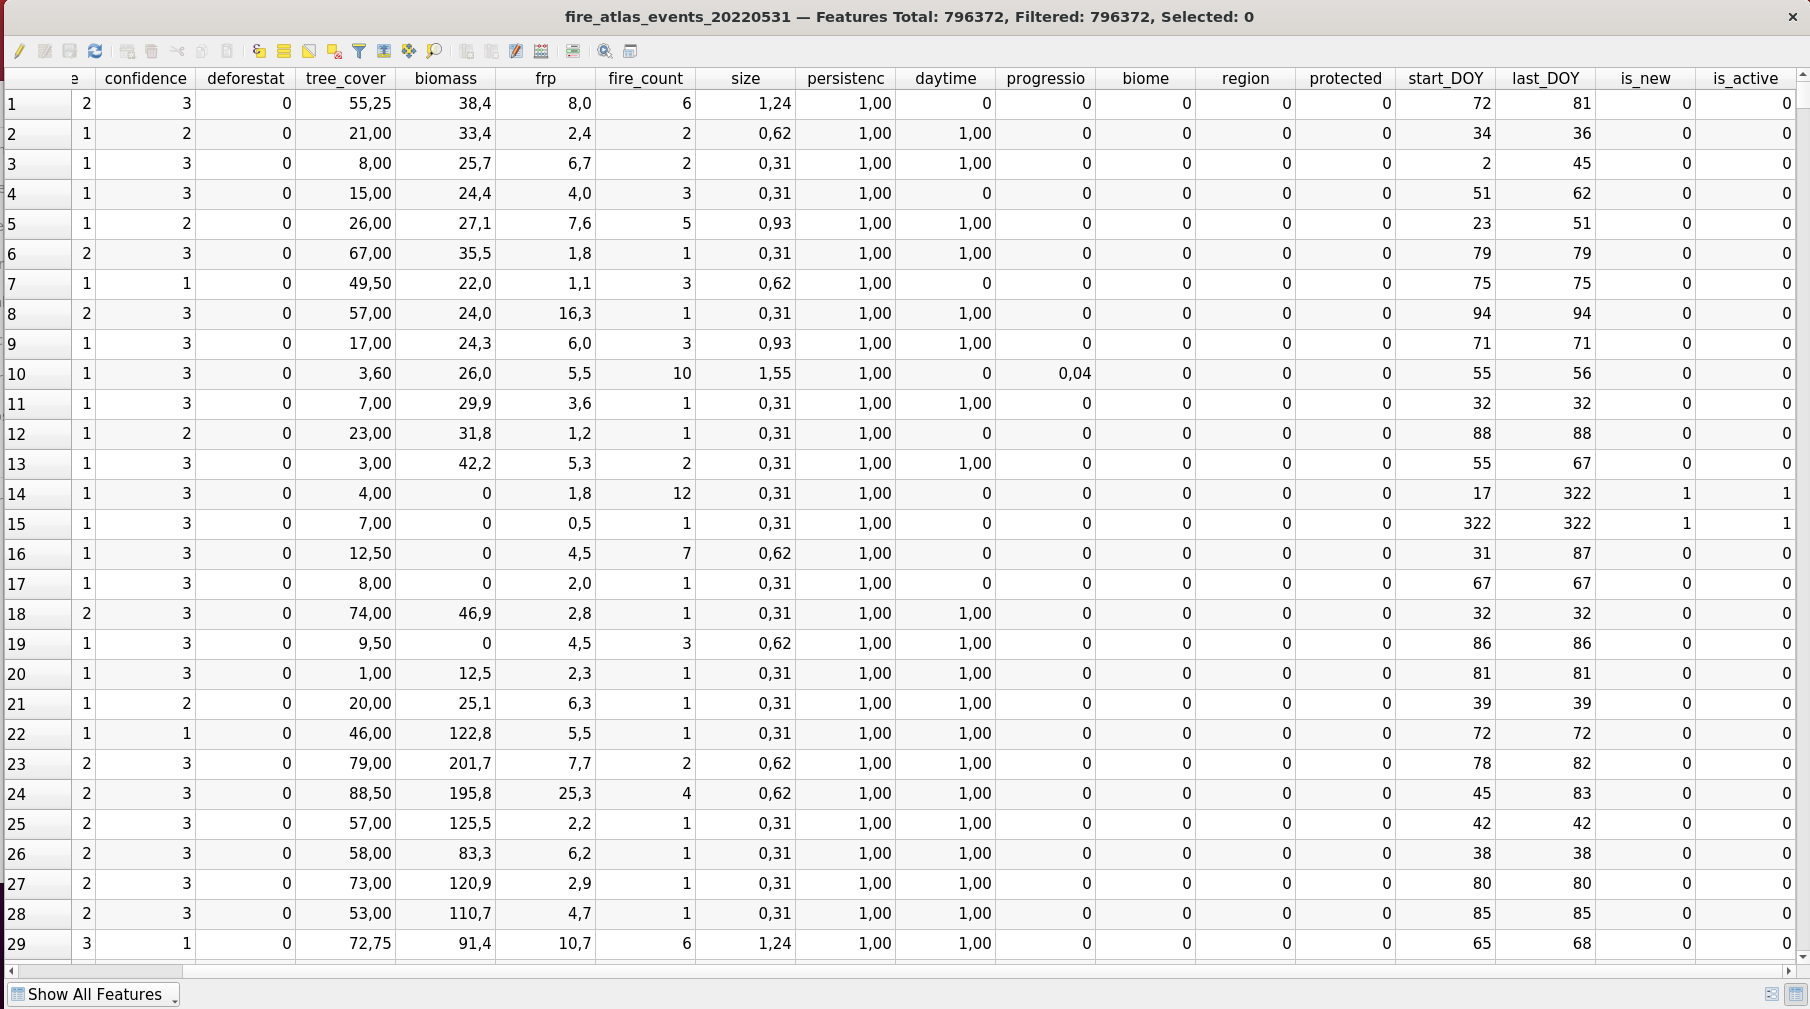
\includegraphics[width=\linewidth]{tg1/figuras/tabela_atributos.png}
		\caption{Tabela de atributos do \textit{shapefile}} \label{fig:tabat}
	\end{minipage}
\end{figure}

\newpage

\begin{multicols}{2}
    

\begin{itemize}
    \item \textbf{fire\_type:} tipo de fogo - (1) savana e pastagem, (2) pequenas clareiras, (3) sub-bosque, (4) desmatamento;
    \item \textbf{confidence:} confiança - (1) baixa, (2) moderada, (3) alta;
    \item \textbf{tree\_cover:} fração média de cobertura arbórea dentro do perímetro (\%);
    \item \textbf{biomass:} biomassa média dentro do perímetro do fogo (ton/ha);
    \item \textbf{deforestation:} fração (0-1) de quadrante de 550m com desmatamento histórico (2015-2019);
    \item \textbf{size:} tamanho do fogo em $km^2$;
    \item \textbf{detections:} número total de detecções dentro do período;
    \item \textbf{frp:} potência radiativa média de fogo (FRP) em megawatts (MW).  Trata-se de uma técnica para quantizar biomassa queimada medindo a radiação de energia infravermelha \cite{NASAMODIS};
    \item \textbf{persistence:} persistência em dias;
    \item \textbf{progression:} fração média de progressão do fogo em quadrantes de 550m (0-1);
    \item \textbf{daytime:} (0) não de dia, (1) de dia;
    \item \textbf{start\_DOY:} dia do início do novo incêndio a partir do dia do ano (1-366);
    \item \textbf{last\_DOY:} detecção de incêndio ativa mais recente a partir do dia do ano (1-366);
    \item \textbf{is\_new:} (1) começou nas últimas 24 horas, (0) incêndio já existente;
    \item \textbf{is\_active:} (1) o fogo estava ativo nos últimos 10 dias (0) ou não;
    \item \textbf{biome:} (1) o fogo está dentro (0) ou fora do bioma Amazônia;
    \item \textbf{protected:} fração (0-1) de fogo ocorrendo dentro de área protegida ou terra indígena;
    \item \textbf{region:} (0-21) qual a região do evento do fogo.
\end{itemize}
\end{multicols}

\subsection{\textit{Dataframe}}

Para converter o conteúdo da tabela de atributos em um \textit{dataframe}, faz-se necessário o uso das bibliotecas \textit{geopandas} e \textit{pandas} do \textit{python}. \textit{Pandas} é uma ferramenta de análise e manipulação de dados, e \textit{geopandas} estende os tipos de dados usados pelos \textit{pandas} para permitir operações espaciais em tipos geométricos. O que fazemos então é primeiro abrir o arquivo do tipo \textit{shapefile} usando \textit{geopandas} para criar um \textit{GeoDataFrame} e então usar uma função da biblioteca \textit{pandas} para convertê-lo em um \textit{dataframe} normal com as \textit{features} que iremos utilizar como entrada para os algoritmos de aprendizado de máquina.

\section{CENSIPAM}
\label{sec:censipamBD}

Assim como o \textit{Amazon Dashboard}, o banco de dados obtido pelo CENSIPAM está em formato \textit{shapefile}. Tal banco pode ser acessado através do recurso de adição de camadas Web Feature Service (WFS) no QGIS, utilizando uma URL específica que aponta para um serviço remoto contendo dados vetoriais geoespaciais. O WFS é um padrão da Open Geospatial Consortium (OGC) que define interfaces para servir e consumir dados geoespaciais vetoriais pela web.

Na figura \ref{fig:qgiscensipam} temos um exemplo do que podemos visualizar ao acessar o banco de dados do CENSIPAM pelo QGIS:

\begin{figure}[htb]
	\centering
	\begin{minipage}{0.6\linewidth}
		\centering
		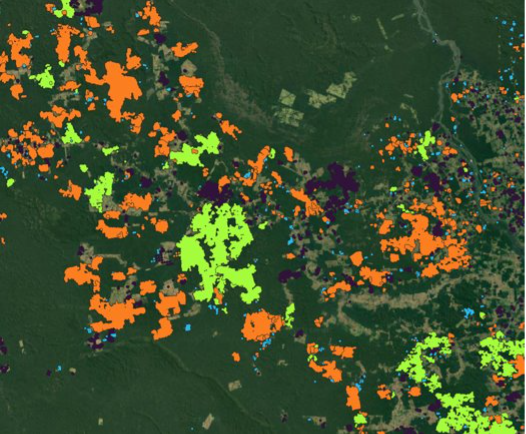
\includegraphics[width=\linewidth]{tg1/figuras/mapa_censipam.png}
		\caption{Mapa no QGIS com eventos de fogo} \label{fig:qgiscensipam}
	\end{minipage}
\end{figure}

Uma adição interessante presente nos dados do CENSIPAM se comparados com os do GFED, é a capacidade de adquirirmos diversas detecções de um mesmo evento de fogo como demonstrado na figura \ref{fig:progressao}. Com o GFED tinhamos acesso apenas a classificação e \textit{features} mais recente do incêndio, referente a sua última detecção realizada, porém com o CENSIPAM podemos obter ambos para detecções passadas, o que abre a possibilidade de incluir as características dinâmicas e temporais da queimada na sua classificação.



\begin{figure}[htb]
	\centering
	\begin{minipage}{0.9\linewidth}
		\centering
		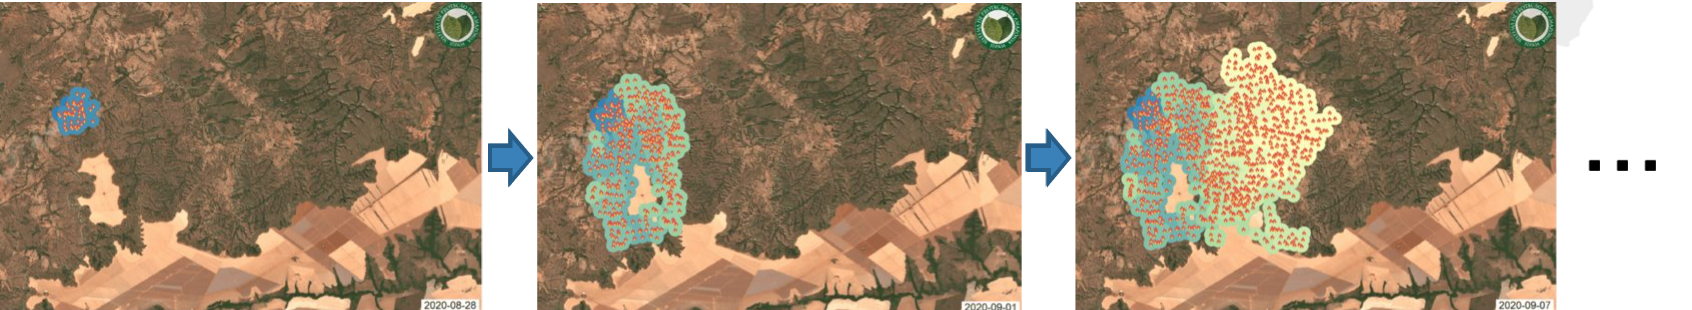
\includegraphics[width=\linewidth]{tg1/figuras/progressao_queimada.png}
		\caption{Ilustrações demonstrativas do crescimento de um evento de fogo ao longo do tempo} \label{fig:progressao}
	\end{minipage}
\end{figure}

Da tabela de atributos destes \textit{shapefiles}, utilizamos as seguintes colunas para o treinamento:

\newpage

\begin{multicols}{2}
    


\begin{itemize}
\item \textbf{id\_evento}: Representa o código de identificação interno de um evento de fogo catalogado pelo sistema. Detecções distintas mas consideradas como um mesmo evento recebem a mesma identificação.
\item \textbf{delta\_area}: Variação da área coberta pelo incêndio em kilometros quadrados.
\item \textbf{q\_focos}: Quantidade de focos de incêndio detectados pelo sistema como pertencendo ao mesmo evento de fogo.
\item \textbf{qtd\_passagens\_com\_deteccao}: Quantas passagens de satélites ocorreram por este evento. Como se trata de 4 pares de satélite em órbitas polares, pode-se ter até 8 detecções por dia \cite{painel-fogo}.
\item \textbf{frp\_med}: \textit{Fire Radiative Power} ou FRP, um dado relativo ao sensor MODIS (\textit{Moderate Resolution Imaging Spectroradiometer}).
\item \textbf{area\_passagem}: Área coberta pelo incêndio no momento da detecção;
\item \textbf{delta\_t\_horas}: Tempo acumulado em horas entre detecções.
%\item \textbf{p\_norm}:
\item \textbf{ve\_expansao}: Velocidade estimada de expansão do incêndio.

\end{itemize}

\end{multicols}

\section{Análise das \textit{features} do GFED}
\label{sec:features}

Ao todo são utilizadas 17 \textit{features} diferentes para realizarmos a classificação do tipo de fogo, que estão descritas na subseção \ref{sec:shp} (cluster\_ID não é utilizado). Nem sempre todas as informações que entregamos para um algoritmo de aprendizado de máquina são úteis para a previsão, o que explica não utilizarmos o cluster\_ID, pois se cada evento de fogo possui um número de identificação diferente, esse número nada diz a respeito sobre qual o tipo de queimada que ocorreu. Podemos fazer uma correlação entre cada tipo de dado fornecido e os tipos de fogo, observando assim quais informações são mais descritivas para o algoritmo, quais delas são mais úteis para separar os 4 tipos.

Para podermos observar a relação que cada \textit{feature} possui com a saída, foram feitos diversos gráficos de dispersão em 3 dimensões que combinam o efeito que até 3 \textit{features} em conjunto podem ter para separar cada tipo de queimada em nuvens. Os gráficos estão dispostos nas figuras a seguir:


\begin{multicols}{2}

\begin{figure}[H]
    \caption{Start day x Is new x Is active}
     
    \centering 
    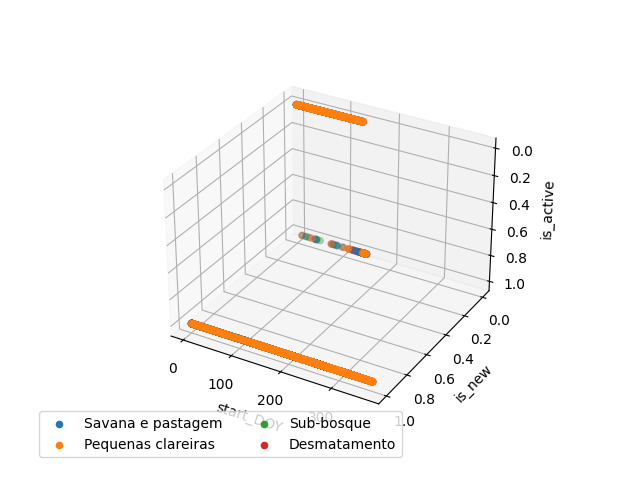
\includegraphics[width=0.9\linewidth]{tg1/figuras/start_DOYxis_newxis_active--150--120.png}
    \label{figura:six}
\end{figure}

\begin{figure}[H]
    \caption{Biome x Region x Protected}
     
    \centering 
    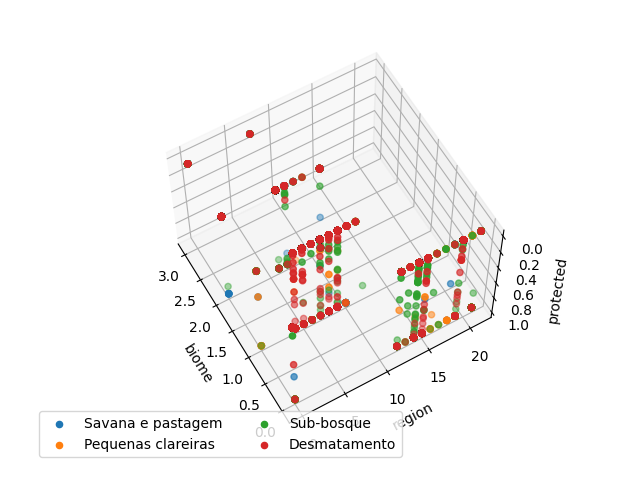
\includegraphics[width=1.1\linewidth]{tg1/figuras/biomexregionxprotected--120-30.png}
    \label{figura:one}
\end{figure}
        
\begin{figure}[H]
    \caption{Biome x Region x Protected}
     
    \centering 
    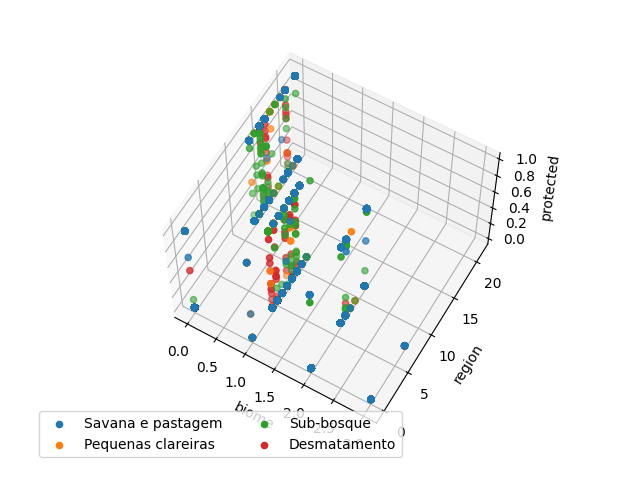
\includegraphics[width=1.1\linewidth]{tg1/figuras/biomexregionxprotected-60--60.png}
    \label{figura:two}
\end{figure}

\begin{figure}[H]
    \caption{Deforestat x Tree cover x Biomass}
     
    \centering 
    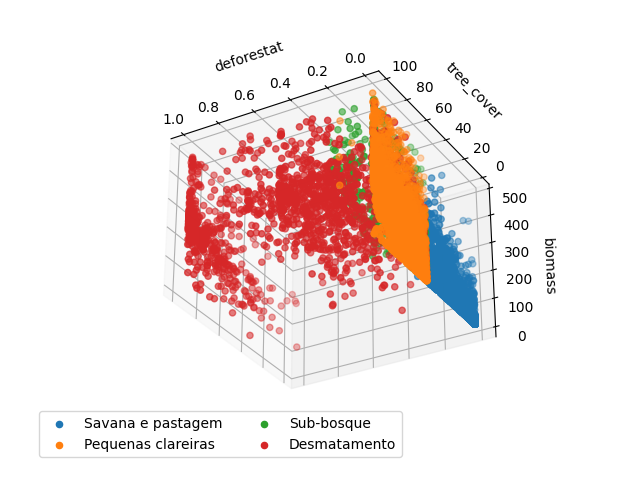
\includegraphics[width=1.1\linewidth]{tg1/figuras/deforestatxtree_coverxbiomass---30--120.png}
    \label{figura:three}
\end{figure}

\begin{figure}[H]
    \caption{FRP x Detections x Size}
     
    \centering 
    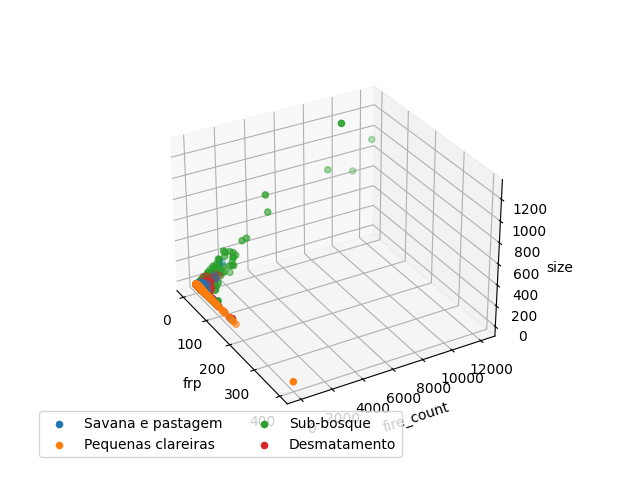
\includegraphics[width=1.1\linewidth]{tg1/figuras/frpxfire_countxsize-30--30.png}
    \label{figura:four}
\end{figure}

\begin{figure}[H]
    \caption{Persistence x Daytime x Progression}
     
    \centering 
    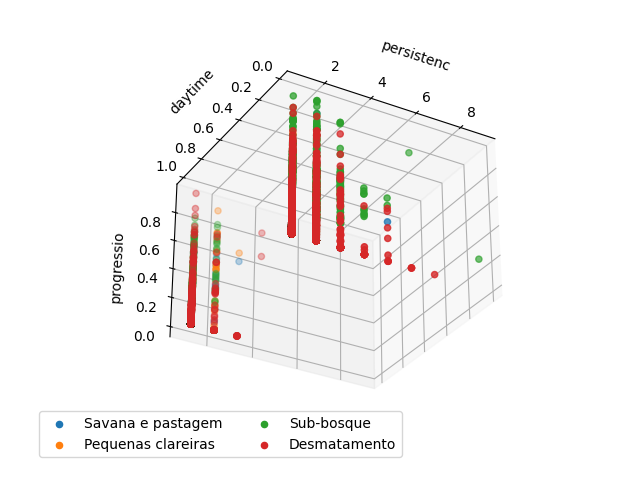
\includegraphics[width=1.1\linewidth]{tg1/figuras/persistencxdaytimexprogressio--30--120.png}
    \label{figura:five}
\end{figure}

\begin{figure}[H]
    \caption{Start day x Is new x Is active}
     
    \centering 
    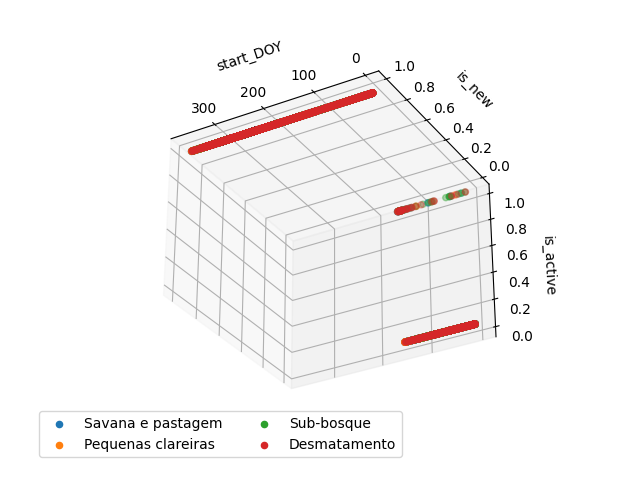
\includegraphics[width=1.1\linewidth]{tg1/figuras/start_DOYxis_newxis_active--30-120.png}
    \label{figura:seven}
\end{figure}
            
\end{multicols}

Podemos observar através dos gráficos que os tipos de fogo de savana (0) e pequenas clareiras (1) são mais fáceis de se tipificar, dados como \textit{tree cover}, \textit{deforestat}, \textit{frp}, \textit{fire count} e \textit{biomass} em conjunto são capazes de delimitar fortemente esses dois tipos. O desmatamento (4) e sub-bosque (3) apresentam maior diluição um com o outro e com os outros tipos, o que explica a maior dificuldade dos algoritmos em prevê-los corretamente, como será visto no capítulo \ref{resultados}.

Como podemos ver na seção \ref{sec:censipamBD}, o banco de dados do CENSIPAM não conta com boa parte das \textit{features} presentes no banco do GFED, e como podemos ver algumas delas se mostraram essenciais para acusação do tipo do fogo. Torna-se necessário então buscar outras fontes que forneçam tais informações.

%\todo[inline]{}

\section{Adição de \textit{features}}
%Dos dados listados acima, apenas 18 são disponibilizados diretamente pelos servidores do CENSIPAM. Os demais dados têm de ser produzidos a partir de outros conjuntos de dados disponibilizados por diferentes entidades. 

A produção destes dados para a adição ao banco do CENSIPAM envolve o cruzamento com dados de diversas outras entidades. Sua produção se dá pelo cálculo da intersecção geográfica dos eventos de fogo e diversos mapas disponibilizadas pelas entidades Terrabrasilis \cite{terrabrasilis}, MapBiomas \cite{MapBiomasQueimadas} e GFED \cite{gfed}.

A partir das coordenadas dos focos de incêndio, é possível de se fazer uma comparação com outros mapas para se encontrar intersecções com áreas de interesse. Por exemplo, dados relativos à proximidade à áreas de conservação ambiental e áreas indígenas são produzidos pelo cruzamento com os dados disponíveis pelo Terrabrasilis. Já informações como desmatamento da área podem ser obtidas por meio do DETER \cite{deter}, enquanto informações Áreas Públicas, Privadas, Desconhecidas e Áreas de Cadastro Ambiental Rural são obtidas a partir do Cadastro Ambiental Rural \cite{cadastro-rural}.

 O código de aquisição e cruzamento foi feito com base no modelo desenvolvido por Bruno Scholles \cite{BrunoScholess2023}, por meio do qual foi-se possível adicionarmos as seguintes \textit{features} ao \textit{dataframe}:

\begin{figure}[htb]
	\centering
	\begin{minipage}{0.9\linewidth}
		\centering
		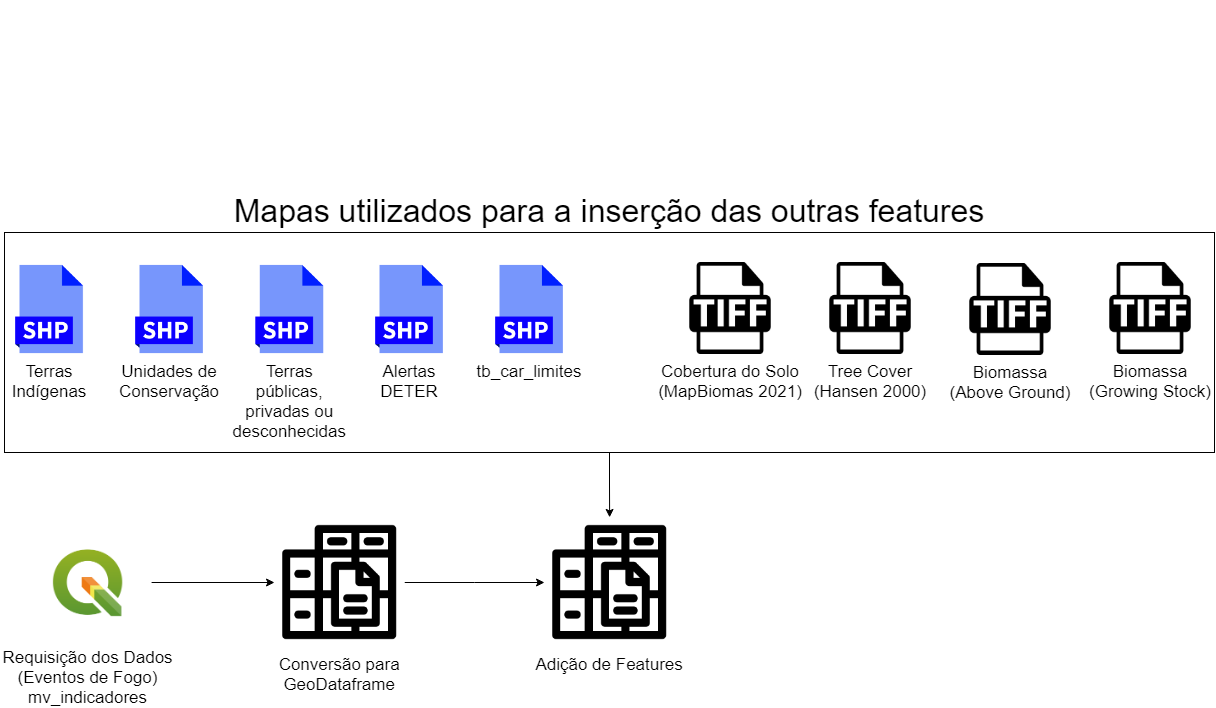
\includegraphics[width=\linewidth]{tg1/figuras/esquematico_banco.png}
		\caption{Esquemático do processo de obtenção de \textit{features}} \label{fig:featuresextras}
	\end{minipage}
\end{figure}
\begin{multicols}{2}
    \begin{itemize}
\item \textbf{areakm2\_UC}: Área em $km^2$ da detecção pertencente à uma unidade de conservação;
\item \textbf{perc\_in\_UC}: Porcentagem da área da detecção da detecção pertencente à uma unidade de conservação;
\item \textbf{areakm2\_IN}:Área em $km^2$ da detecção pertencente à território indígena;
\item \textbf{perc\_in\_IN}:Porcentagem da área da detecção da detecção pertencente à território indígena;
\item \textbf{deter\_area}:Área em $km^2$ da detecção pertencente à área em que ocorreu desmatamento;
\item \textbf{deter\_days}: Quantidade de dias passados desde a demarcação do DETER como área em que ocorreu desmatamento; 
\item \textbf{deter\_perc}:Porcentagem da área da detecção da detecção pertencente à área em que ocorreu desmatamento;
\item \textbf{tree\_cover}: Cobertura de árvore, métrica referente à porcentagem da área que é coberta por copas de árvores ou vegetação alta.
\item \textbf{a\_cover\_X e p\_cover\_X (onde X pode ser 3, 4, 5, 9, 11, 12, 15, 20, 21, 23, 24, 25, 29, 30, 32, 33, 39, 40, 41, 48, 62)}: Cobertura do solo (tipo de vegetação) medida em área e porcentagem;
\item \textbf{biomass\_AG}: biomassa \textit{Above Ground} média dentro do perímetro
\item \textbf{biomass\_GS}: biomassa \textit{Growing Stock} média dentro do perímetro
\item \textbf{a\_terr\_pri e p\_terr\_pri}: Perímetro da detecção pertencente à área privada;
\item \textbf{a\_terr\_pub e p\_terr\_pub}: Perímetro da detecção pertencente à área pública;
\item \textbf{a\_terr\_unk e p\_terr\_unk}: Perímetro da detecção pertencente à área não classificada como pública ou privada (\textit{unknown});
\item \textbf{area\_CAR e per\_car}: Perímetro da detecção pertencente à área de Cadastro Ambiental Rural;
\end{itemize}
\end{multicols}





\chapter{Resultados}
\label{resultados}

\section{GFED}

\subsection{\textit{Random Forest}}

\textit{Random Forest} é um dos modelos de algoritmo mencionado no capítulo 3. Modelos
\textit{Random Forest} são escolhidos para produzir boas previsões que são fáceis de entender. O fato de que pode lidar com grandes conjuntos de dados com eficiência e fornecer um alto nível de precisão geral é uma das razões pelas quais o escolhemos para verificar a eficácia de técnicas de aprendizado de máquina dentro do nosso problema.

\subsection{\textit{Multi-Layer Perceptron}}

MLP é um modelo de perceptron mencionado no capítulo 3. Esta arquitetura é muito
configurável, principalmente quando construída a partir de um \textit{framework} como o Pytorch. No entanto, esta maleabilidade também proporciona muitos pontos de falha, como bugs ou dificuldades de implementação.

Redes como o MLP tendem a lidar melhor com dados contínuos e a terem dificuldades
em interpretar dados categóricos, o que traz outros desafios na adaptação do conjunto de
dados para esta arquitetura.

\subsection{Metodologia}

Podemos descrever o funcionamento do códigos de treinamento dos modelos por meio do seguinte fluxograma, na figura \ref{fig:rfflux}:

\begin{figure}[H]
	\centering
	\begin{minipage}{0.98\linewidth}
		\centering
		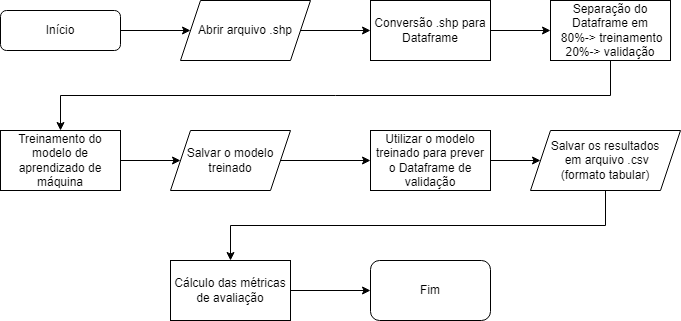
\includegraphics[width=\linewidth]{tg1/figuras/fluxograma_gfed.png}
		\caption{Fluxograma do funcionamento dos códigos de treinamento} \label{fig:rfflux}
	\end{minipage}
\end{figure}

Os parâmetros utilizados para a função do \textit{Random Forest Classifier} foram os valores padrões utilizados pelo scikit-learn \cite{sklearnrfc}, com o objetivo de obter-se um primeiro resultado para o nosso modelo. Enquanto os parâmetros do MLP foram sendo definidos até que a rede apresentasse \textit{overfitting}, demonstrando capacidade de generalização. Após isto, os seus hiper-parâmetros foram ajustados até fossem atingidos os melhores resultados encontrados.

\subsection{Desempenho}

Na última etapa de calculo da precisão do modelo Random Forest, foi obtido os
valores da tabela \ref{tab:rf} para quando classificamos o dataframe de validação. Já os valores para o MLP estão dispostos na tabela \ref{tab:mlp}.

\begin{table}[H]
\centering
\caption{Precisão do Modelo Random Forest}
\label{tab:rf}
\begin{tabular}{lllll}
Classe           & Precision & Recall & F1-score & Support \\
0                & 1.00      & 1.00   & 1.00     & 124125  \\
1                & 1.00      & 1.00   & 1.00     & 29652   \\
2                & 0.84      & 0.73   & 0.78     & 1866    \\
3                & 0.86      & 0.92   & 0.89     & 3615    \\  \cline{1-1}
Acurácia         &           &        & 0.99     & 159258  \\
Média aritmética & 0.92      & 0.91   & 0.92     & 159258  \\
Média ponderada  & 0.99      & 0.99   & 0.99     & 159258 
\end{tabular}
\end{table}

\begin{table}[H]
\centering
\caption{Precisão do modelo MLP}
\label{tab:mlp}
\begin{tabular}{lllll}
Classe          & Precision & Recall & F1-score & Support \\
0               & 1.00      & 1.00   & 1.00     & 124125  \\
1               & 0.98      & 1.00   & 0.99     & 29652   \\
2               & 0.69      & 0.66   & 0.68     & 1866    \\
3               & 0.79      & 0.84   & 0.81     & 3615    \\ \cline{1-1}
Média ponderada & 0.99      & 0.99   & 0.99     & 159258 
\end{tabular}
\end{table}

\subsection{Conclusões}

Os resultados obtidos por meio da aplicação de dois modelos distintos de aprendizado de máquina, Random Forest e Multi-Layer Perceptron (MLP), na tarefa de classificação de queimadas na Amazônia, revelaram-se altamente promissores. Ambos os modelos demonstraram uma capacidade robusta de aprender padrões complexos nos dados, contribuindo para uma precisão notável na identificação de áreas afetadas por queimadas. Esses resultados preliminares destacam o potencial dessas técnicas de aprendizado de máquina na monitorização e prevenção de eventos de queimadas na Amazônia, representando um avanço significativo na aplicação de soluções inovadoras para desafios ambientais complexos.

Confirmada a eficácia da utilização de \textit{machine learning} para o banco de dados do GFED, podemos então trazer nossa metodologia para o banco de dados do Censipam, sobre o qual o nosso trabalho deverá operar para ser integralizado ao Painel do Fogo, trazendo também as \textit{features} de maior importância, as quais foram obtidas conforme está descrito na seção \ref{sec:features}.

Em Bruno Scholles \cite{BrunoScholess2023} pode-se observar o desempenho do algoritmo de \textit{Random Forest} para a base de dados do Painel do Fogo. O trabalho aqui apresentado procura usufruir da vantagem fornecida de datação separada para cada detecção do evento dentro dessa base assim como ilustrado na figura \ref{fig:progressao}. Graças a isso, é possível testarmos a eficiência de um modelo do tipo LSTM para realizar a classificação de queimadas, analisando-as como uma série temporal.



\section{LSTM}
%\todo[inline]{print do código no tema claro, com huperparâmetros}

\subsection{Modelo}

Abaixo encontra-se o código em Python da implementação de um módulo LSTM por meio do Pytorch.

\begin{figure}[ht]
    \centering
    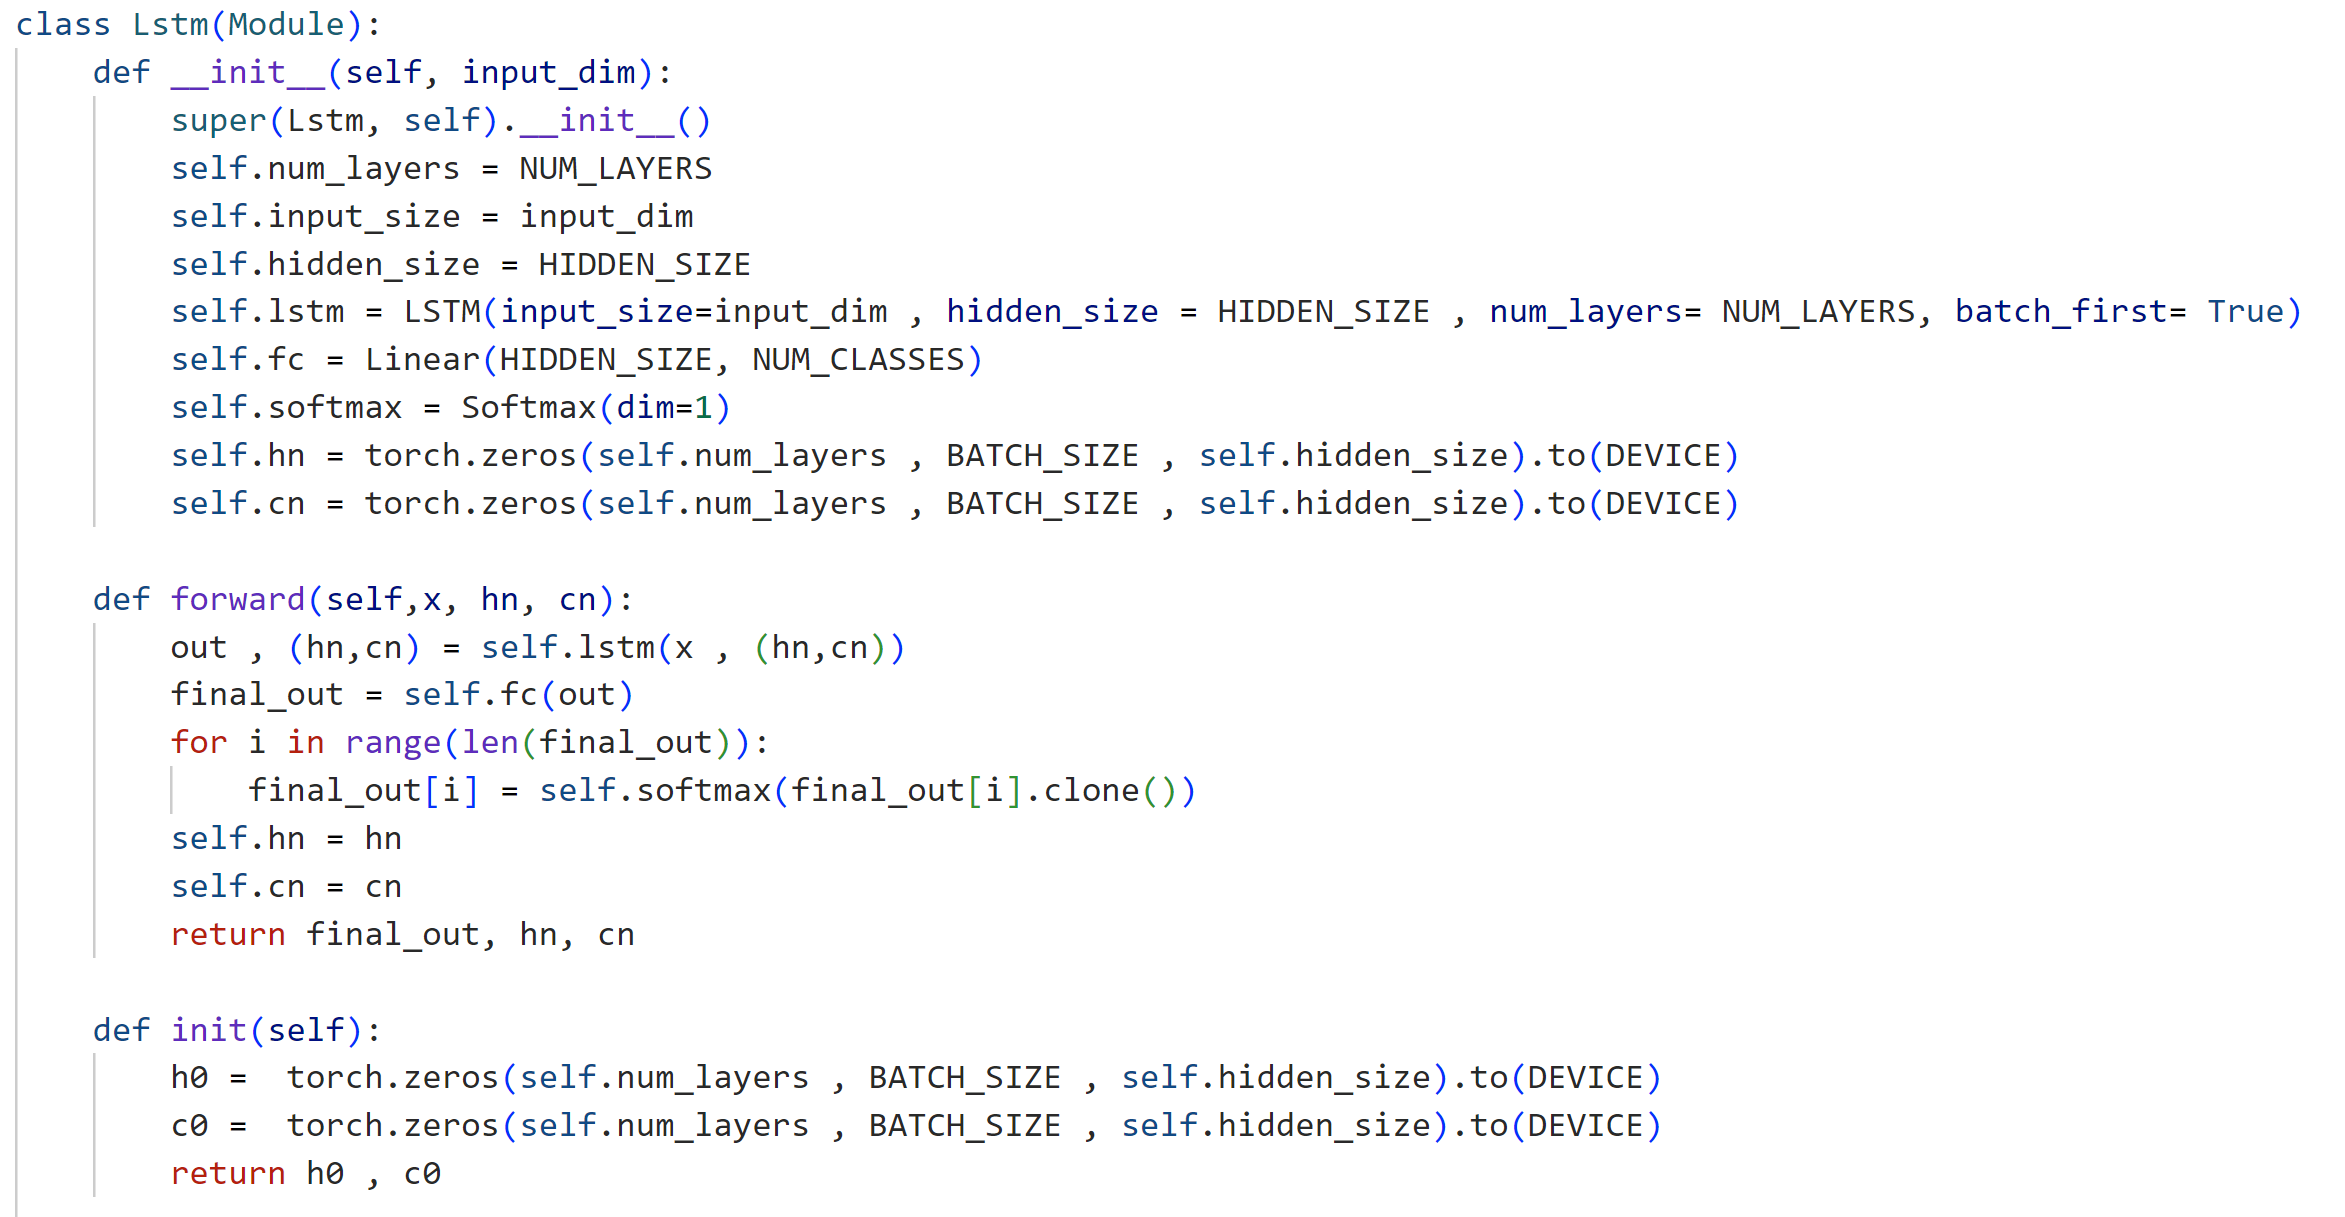
\includegraphics[scale=0.5]{tg1/figuras/codigo.png}
    \caption{Código do modelo LSTM}
    \label{fig:codigo_lstm}
\end{figure}

Os hiperparâmetros são:
\begin{table}[h]
    \centering
    \begin{tabular}{|l|c|l|}
        \hline
        \textbf{Parâmetros} & \textbf{Significado} & \textbf{Valor} \\
        \hline
        NUM\_LAYERS & Número de camadas & 2 \\
        input\_dim & Dimensão da entrada (número de features) &  68\\
        HIDDEN\_SIZE & Tamanho do estado oculto &  60\\
        \hline
    \end{tabular}
    \caption{Parâmetros do Modelo}
    \label{tab:hiperparametros}
\end{table}

Abaixo encontra-se o código do algoritmo de \textit{loss} implementada via Pytorch \cite{Lin_Goyal_Girshick_He_Dollar_2017}.

\begin{figure}[ht]
    \centering
    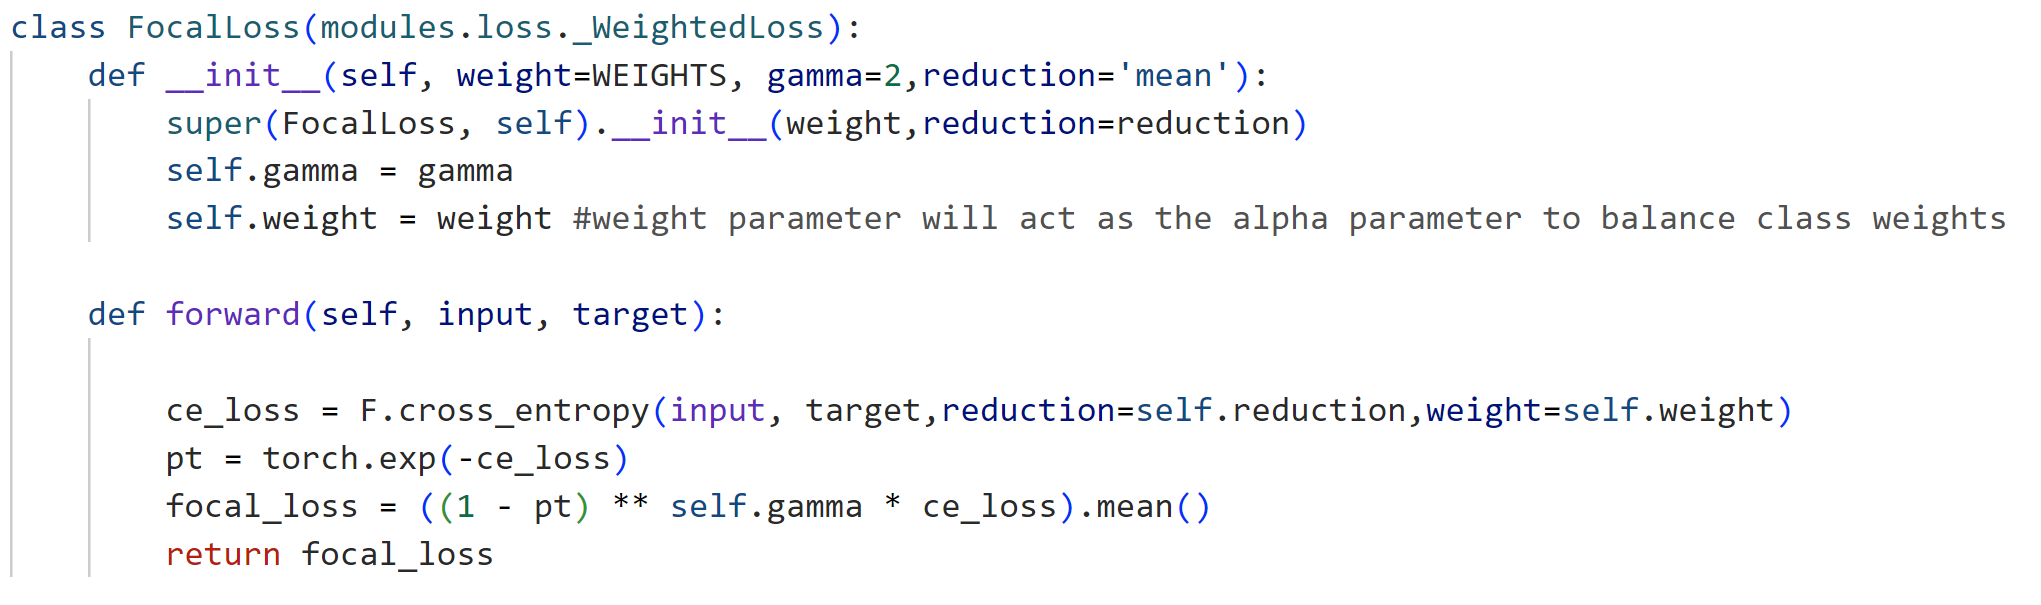
\includegraphics[scale=0.5]{tg1/figuras/loss.png}
    \caption{Código do modelo de Loss Focal}
    \label{fig:loss}
\end{figure}

\subsection{Lidando com Overfitting}
O problema de overfitting foi encontrado durante alguns testes como consequência do mal balanceamento do dataset. A classe 3, referente às queimadas de sub-bosque, representa 1.8\% do dataset, o que resulta em 0\% de acurácia para esta classe para um modelo treinando sem qualquer algoritmo de balanceamento.

É comum na literatura encontrar exemplos de "data augmentation" \cite{survey_data_augmentation}. Trata-se de algoritmos capaz de expandir um dataset sem comprometer de forma significativa seu valor como dado de treinamento. Neste trabalho, optou-se por empregar uma redução de dados como estratégia de balanceamento. Esta estratégia envolve eliminar de forma aleatória dados de rótulos diferentes de forma a se aumentar a representação do tipo de dados de menor presença no dataset. Este tipo de estratégia acabou resultando em overfitting, conforme a imagem a seguir.

\begin{figure}[ht]
    \centering
    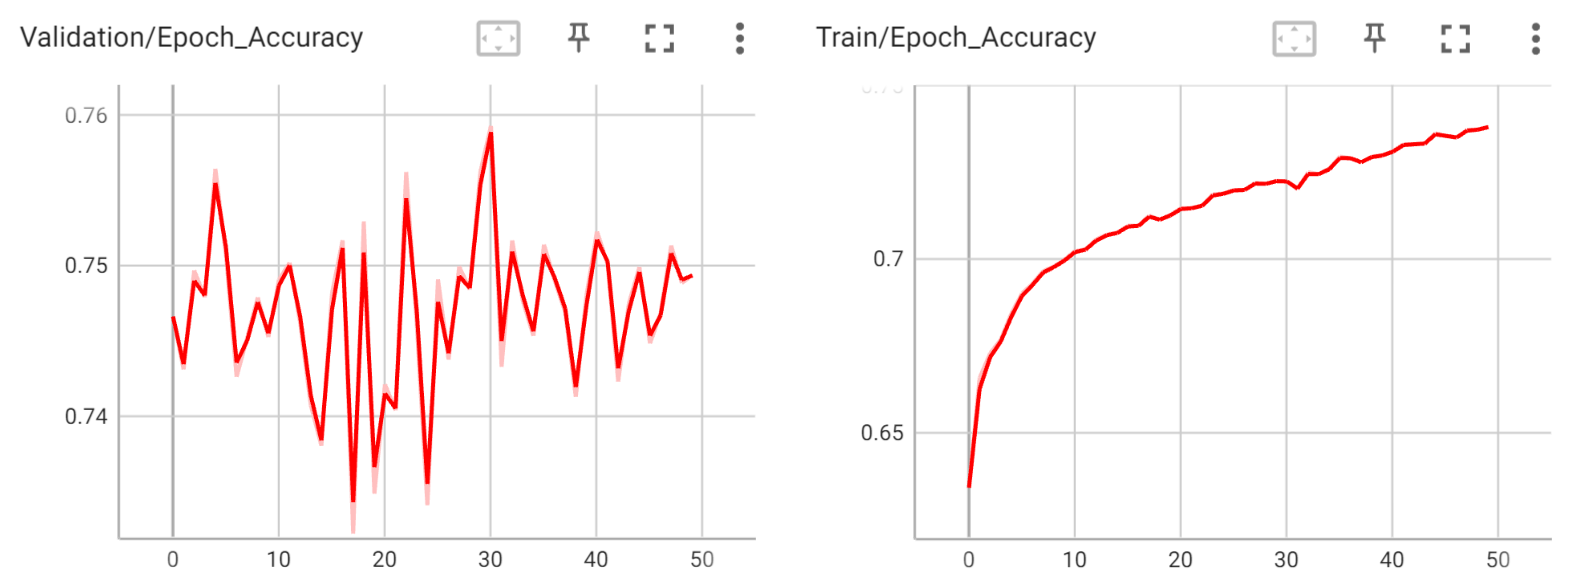
\includegraphics[scale=0.5]{tg1/figuras/overfit.png}
    \caption{Overfitting no treinamento}
    \label{fig:overfitting}
\end{figure}

Na figura \ref{fig:overfitting} pode-se ver que embora a acurácia de treinamento esteja aumentando, a acurácia de validação não está melhorando. Dessa forma, pode-se dizer que a rede está se tornando "viciada" nos dados de treinamento, aprendendo a interpretá-los bem mas não se tornando capaz de prever dados diferentes deste.

Tendo em mãos estes resultados, optou-se por utilizar um leve balanceamento, aumentando a representatividade de 1.8\% para 5\%. Esta proporção foi obtida de forma empírica como um valor que representa uma melhora significativa na acurácia para a classe 3 porém sem reduzir demais a acurácia para as demais classes.


\subsection{Organização em Série Temporal}

Transformar os dados existentes em uma série temporal envolve a adição de uma nova dimensão, a temporal. Em termos práticos, isto é efetuado por meio de uma dimensão acrescentada aos tensores dos dados transformando eventos discretos em dados sequenciais. 

Os dados disponibilizados pelo Censipam possuem identificadores rotulados como "id\_evento". Estes códigos agrupam diferentes detecções de incêndios como pertencentes a um mesmo foco de incêndio e é necessário para a transformação dos dados em uma série temporal. Em outras palavras, cada dados possui três dimensões: o ID representando o foco de incêndio, a quantidade de detecções relativas a este mesmo incêndio, e todos os dados de cada uma destas detecções.

No entanto, esta abordagem envolve o desafio de transformar estes dados em tensores. Todo o código utilizado é construído a partir do Pytorch \cite{NEURIPS2019_9015}, que utiliza tensores como tipo de dado. Tensores são matrizes multi-dimensionais, apenas uma forma de se organizar dados de forma lógica. Por exemplo, pode-se imaginar um tensor tridimensional como um cubo, tratando-se de um tensor cujo as três dimensões são iguais.

Em outras palavras, tensores são uma forma de se estruturar dados de forma regular, onde cada amostra de dados possui dimensões constantes e condizentes com as dimensões do tensor. No entanto, os dados em questão não são regulares pois são obtidos a partir de fenômenos aleatórios e caóticos, de queimadas sobre um território florestal de proporções continentais. Por isso é necessário o emprego de alguma técnica de tratamento de dados que possa regularizá-los, permitindo sua manipulação como tensores.

\subsubsection{Padding}

O desafio em questão é transformar dados de comprimento variado em dados padronizados com o mesmo comprimento, para que possam ser organizados como um tensor tridimensional. Dessarte, é necessário de se empregar um algoritmo capaz de preencher lacunas e eliminar excessos para garantir que todos os dados tenham as mesmas proporções.

"\textit{Padding}" não se trata de um algoritmo específico, mas de qualquer algoritmo capaz de preencher lacunas para garantir regularidade entre dados. Tratando-se de séries temporais, os algoritmos de \textit{Padding} mais comuns envolvem preencher com zeros, com médias ou repetindo valores. Neste trabalho, optou-se por preencher as lacunas repetindo-se a última detecção do evento. 

\begin{figure}[ht]
    \centering
    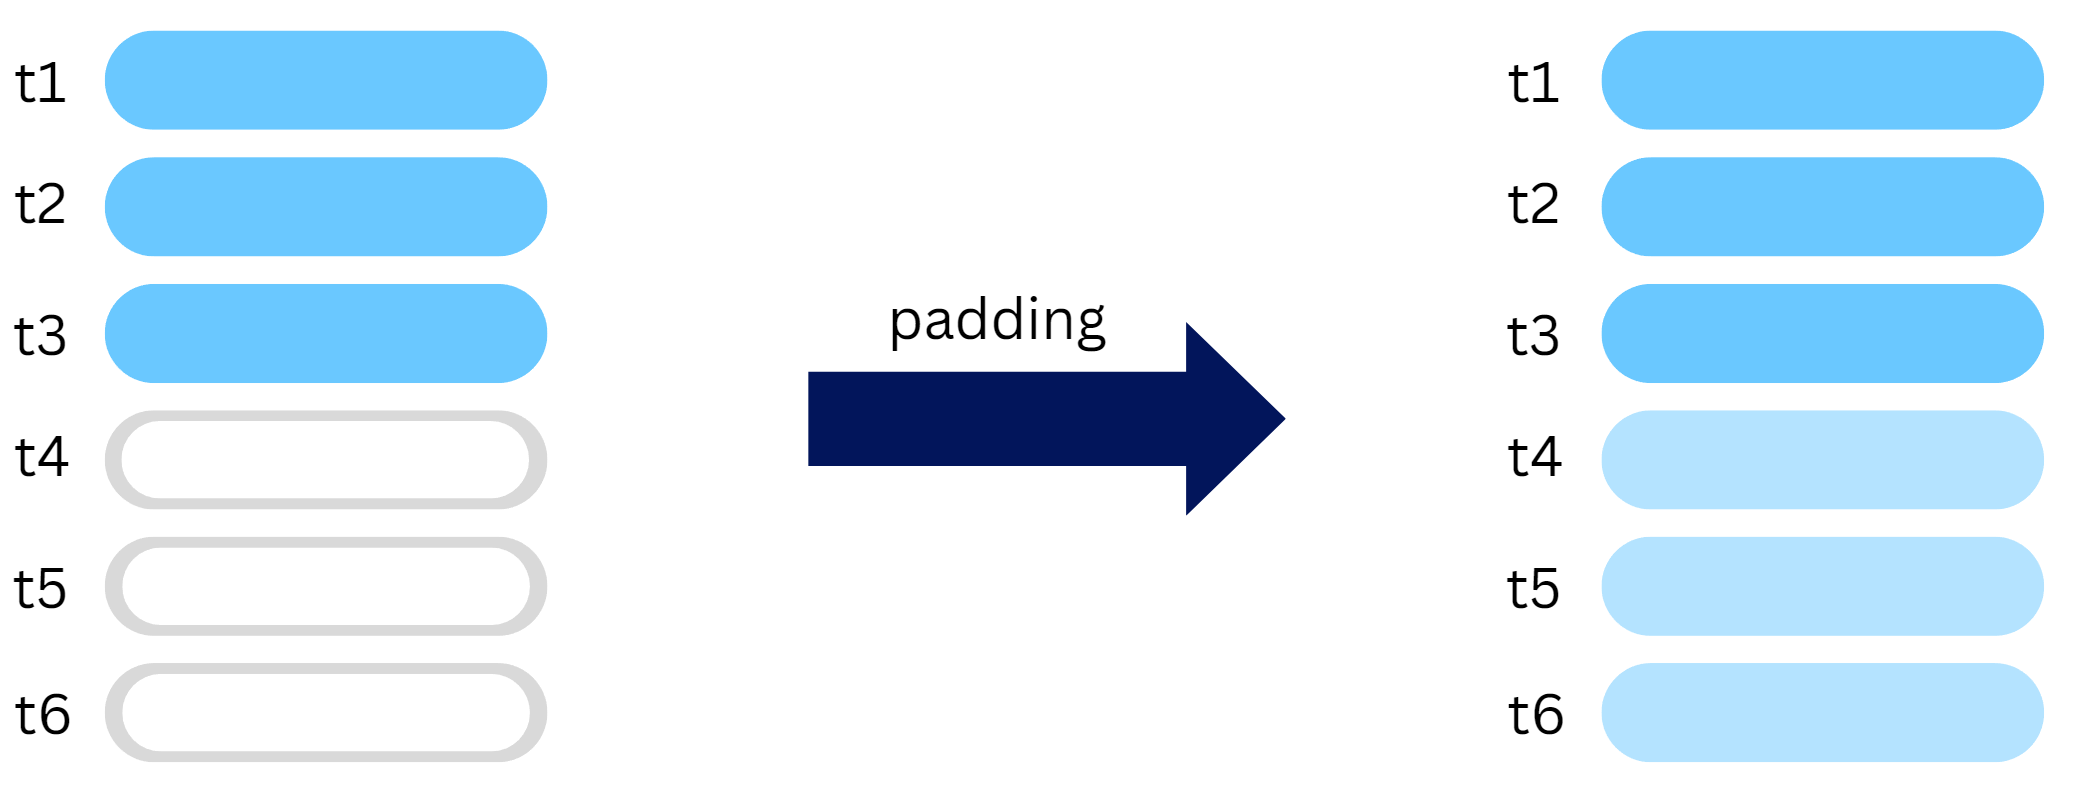
\includegraphics[scale=0.5]{tg1/figuras/padding.png}
    \caption{Representação de Padding}
    \label{fig:padding}
\end{figure}


O motivo para esta escolha é dado pela observação do comportamento da saída da rede ao longo de cada passagem pelos dados. Observou-se que a rede tende ajustar sua saída rapidamente, dentro de 5 iterações, e a manter esta saída até o final, revelando que converge em um valor rapidamente. Logo, foram evitados algoritmos que causem ruído no início da série temporal, período de maior convergência do algoritmo.

\subsection{Metodologia}

Por fim, o funcionamento do código de treinamento pode ser então ilustrado por meio do seguinte fluxograma:
%\todo[inline]{Metodologia toda falando sobre o random forest e nada de lstm, por mim tira esse pedaço e fala sobre LSTM}
%Por meio da biblioteca scikit-learn, é possível escrever um código simples que emprega o uso do modelo Random %Forest e com fácil customização. 

\begin{figure}[H]
	\centering
	\begin{minipage}{0.98\linewidth}
		\centering
		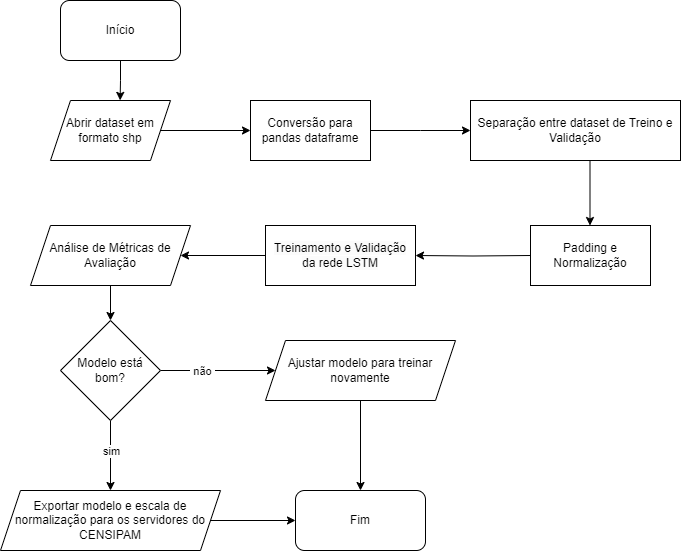
\includegraphics[scale=0.6]{tg1/figuras/flstm_flowchart.png}
		\caption{Fluxograma do funcionamento do código do LSTM} \label{fig:lstm_flowchart}
	\end{minipage}
\end{figure}

\subsection{Desempenho}

No algoritmo de treinamento do modelo, separou-se o dataset entre validação e treinamento, sendo 80\% destinado para o treinamento e 20\% para a validação, separados cronologicamente. As métricas são obtidas de época em época e podem ser observadas por meio do módulo Tensorboard, disponível pelo Tensorflow \cite{tensorflow2015-whitepaper}, ou pelo terminal do programa como uma tabela ao finalizar-se o treinamento, conforme visto na tabela \ref{tab:resultados}.


\todo[inline]{inserir tabela com performance e prints do tensorboard}

    
\begin{table}[h]
    \centering
    \begin{tabular}{|c|c|c|c|c|}
        \hline
        & Acurácia & Precisão & Recall & F1-Score \\
        \hline
        classe 1 & 0.839 & 0.869 & 0.839 & 0.854 \\
        classe 2 & 0.821 & 0.763 & 0.821 & 0.791 \\
        classe 3 & 0 & 0 & 0 & 0 \\
        classe 4 & 0.536 & 0.523 & 0.534 & 0.529 \\
        \hline
        Ponderada & 0.779 & 0.768 & 0.779 & 0.773 \\
        \hline
    \end{tabular}


    \vspace{10pt}
    
    \begin{tabular}{|c|c|}
        \hline
        Classe & Quantidade de eventos \\
        \hline
        classe 1 & 73647 \\
        classe 2 & 64205 \\
        classe 3 & 3136 \\
        classe 4 & 19986 \\
        \hline
    \end{tabular}
    \caption{Resultados da Avaliação}
    \label{tab:resultados}
\end{table}

\subsection{Balanceamento}

Como podemos ver na tabela \ref{tab:resultados}, a rede em seu treinamento praticamente desconsiderou a presença da classe 3 dentro do \textit{dataset}, observando a imagem \ref{fig:lstm_sem_balanc} podemos entender o porque disso. A quantidade de eventos de sub-bosque é bastante inferior a das outras classes, em situações como essa, a rede aprende a não prever aquela classe, isso porque ela é tão inexpressiva que mesmo que ele a desconsidere, a acurácia da rede permanece alta. Como queremos que o trabalho seja capaz de fornecer todas os 4 tipos de fogo, é necessário fazer um balanceamento do \textit{dataset} para aumentar a expressividade das classes menos presentes.

\begin{figure}[H]
	\centering
	\begin{minipage}{0.9\linewidth}
		\centering
		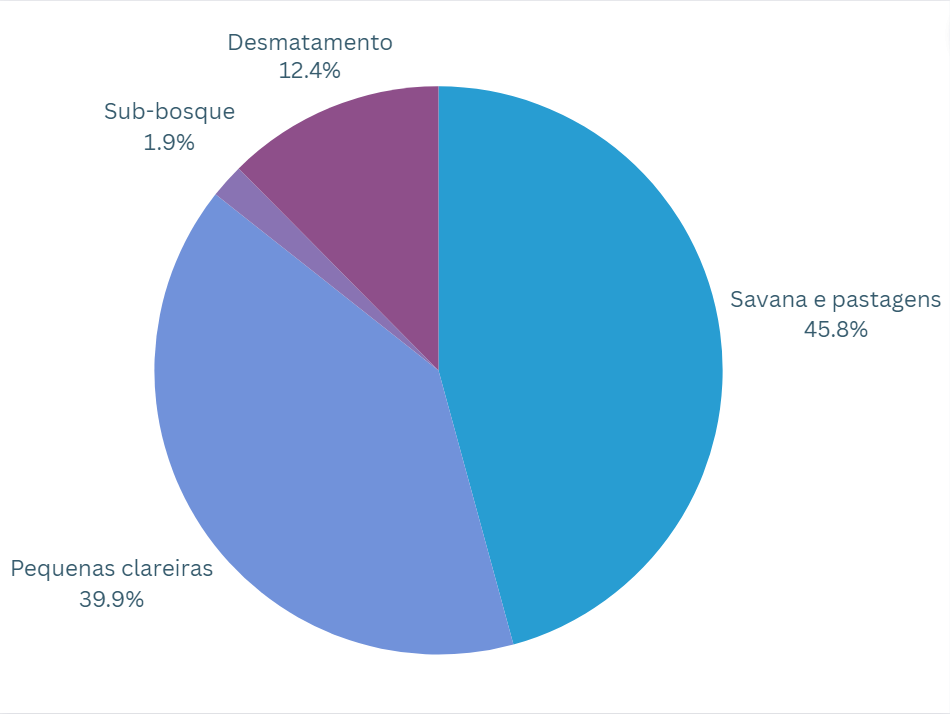
\includegraphics[scale=0.6]{tg1/figuras/sem_balanceamento_pie.png}
		\caption{Gráfico da presença de cada classe dentro do \textit{Dataset}} \label{fig:lstm_sem_balanc}
	\end{minipage}
\end{figure}

O balanceamento pode ser feito utilizando de duas estratégias: remoção de dados e o chamado \textit{data augmentation}, onde aumentamos a quantidade de um certo tipo de dado. Aqui, ambas foram utilizadas, como pode ser observado na tabela \ref{tab:resultados2}, diminuimos a quantidade de eventos para todas as classes exceto a 3, enquanto aumentamos a quantidade de eventos dela. Tal aumento foi feito repetindo os eventos dentro do banco de dados. A tabela também possui o desempenho do modelo para o treinamento com o banco de dados balanceado.

\begin{table}[h]
    \centering
    \begin{tabular}{|c|c|c|c|c|}
        \hline
        & Acurácia & Precisão & Recall & F1-Score \\
        \hline
        classe 1 & 0.795 & 0.904 & 0.795 & 0.846 \\
        classe 2 & 0.804 & 0.772 & 0.804 & 0.788 \\
        classe 3 & 0.290 & 0.237 & 0.289 & 0.261 \\
        classe 4 & 0.620 & 0.485 & 0.619 & 0.544 \\
        \hline
        Ponderada & 0.767 & 0.786 & 0.767 & 0.774 \\
        \hline
    \end{tabular}


    \vspace{10pt}
    
    \begin{tabular}{|c|c|}
        \hline
        Classe & Quantidade de eventos \\
        \hline
        classe 1 & 25088 \\
        classe 2 & 23866 \\
        classe 3 & 9408 \\
        classe 4 & 10662 \\
        \hline
    \end{tabular}
    \caption{Resultados da Avaliação}
    \label{tab:resultados2}
\end{table}

\begin{figure}[H]
	\centering
	\begin{minipage}{0.9\linewidth}
		\centering
		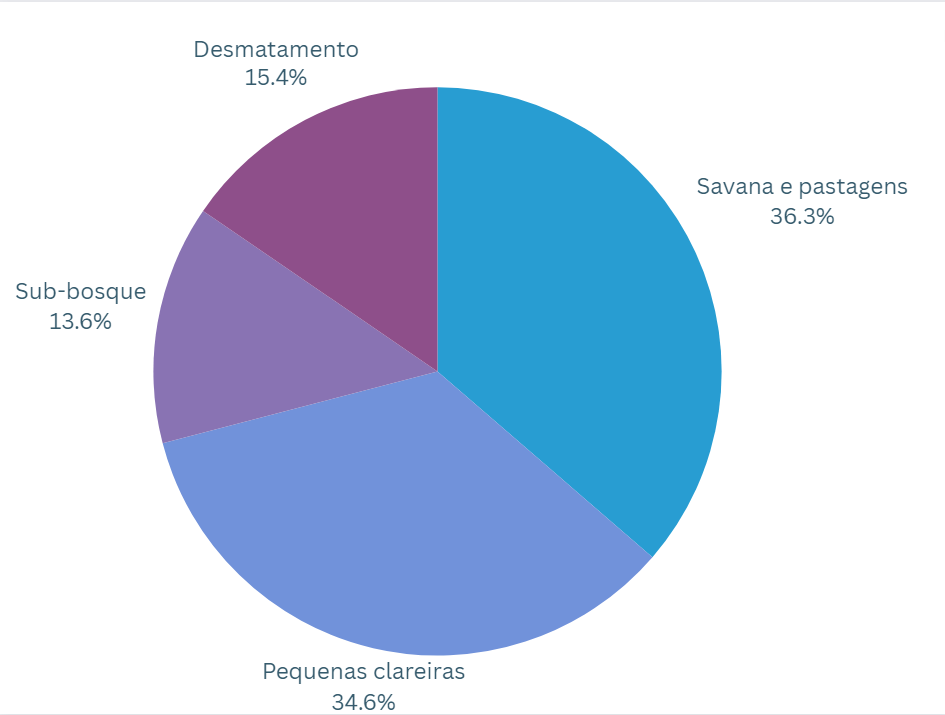
\includegraphics[scale=0.6]{tg1/figuras/balanceado_pie.png}
		\caption{Gráfico balanceado da presença de cada classe dentro do \textit{Dataset}} \label{fig:lstm_com_balanc}
	\end{minipage}
\end{figure}


\section{Servidores do Censipam}

A parceria com o Censipam se deu com o intuito de integrar o modelo de aprendizado como uma ferramenta classificadora em seu sistema. Para isto, foi-se fornecido acesso a uma máquina por meio de tunelamento SSH para que o projeto tenha acesso ao banco de  dados em tempo real.

Dessa forma, o código foi implementado no sistema para que rode continuamente. Atualmente, o programa aguarda até as 23 horas de cada dia para iniciar seu processamento. Neste momento, são requisitados os dados novos, referentes ao dia atual, e os dados antigos de mesmo ID, com apenas XXX features. A partir delas, o algoritmo de adição de features adiciona as demais. Em sequência, os dados passam pela etapa de pré-processamento, sendo normalizados e efetuado o padding. Por fim, o algoritmo de aprendizado de máquina classifica estes dados e monta arquivos dos tipos CSV e SHP com todos os dados classificados.

\subsection{Dados de Treinamento e Dados em Produção}
\todo[inline]{mostrar gráficos comparando ambos datasets}
Os fornecidos para o treinamento do algoritmo e os dados obtidos em produção nos servidores são diferentes. Primeiramente, os dados de treinamento vão até o ano 2022 enquanto os dados disponíveis nos servidores se iniciam em 2023. Além disso, é interessante de se estudar a continuidade entre estes dados, de forma a garantir que sua qualidade é similar à dos dados utilizados no treinamento, ou se houve alguma mudança na forma como são produzidos, como por exemplo, mudança de métrica de metros para quilômetros.


\subsection{Comparando dados do Treinamento com os dados em Produção}

O treinamento do modelo de aprendizado de máquina envolve o uso de um dataset de treino suficientemente parecido com dados de casos práticos, ou aumentam-se as chances de que a performance do modelo em operação não seja satisfatória. Dessa forma, foram-se gerados vários gráficos de caixa comparando as distribuições dos dados utilizados no treinamento com os dados obtidos diretamente dos servidores do Censipam, onde o modelo está em operação diária.

\begin{figure}[H]
	\centering
	\begin{minipage}{0.98\linewidth}
		\centering
		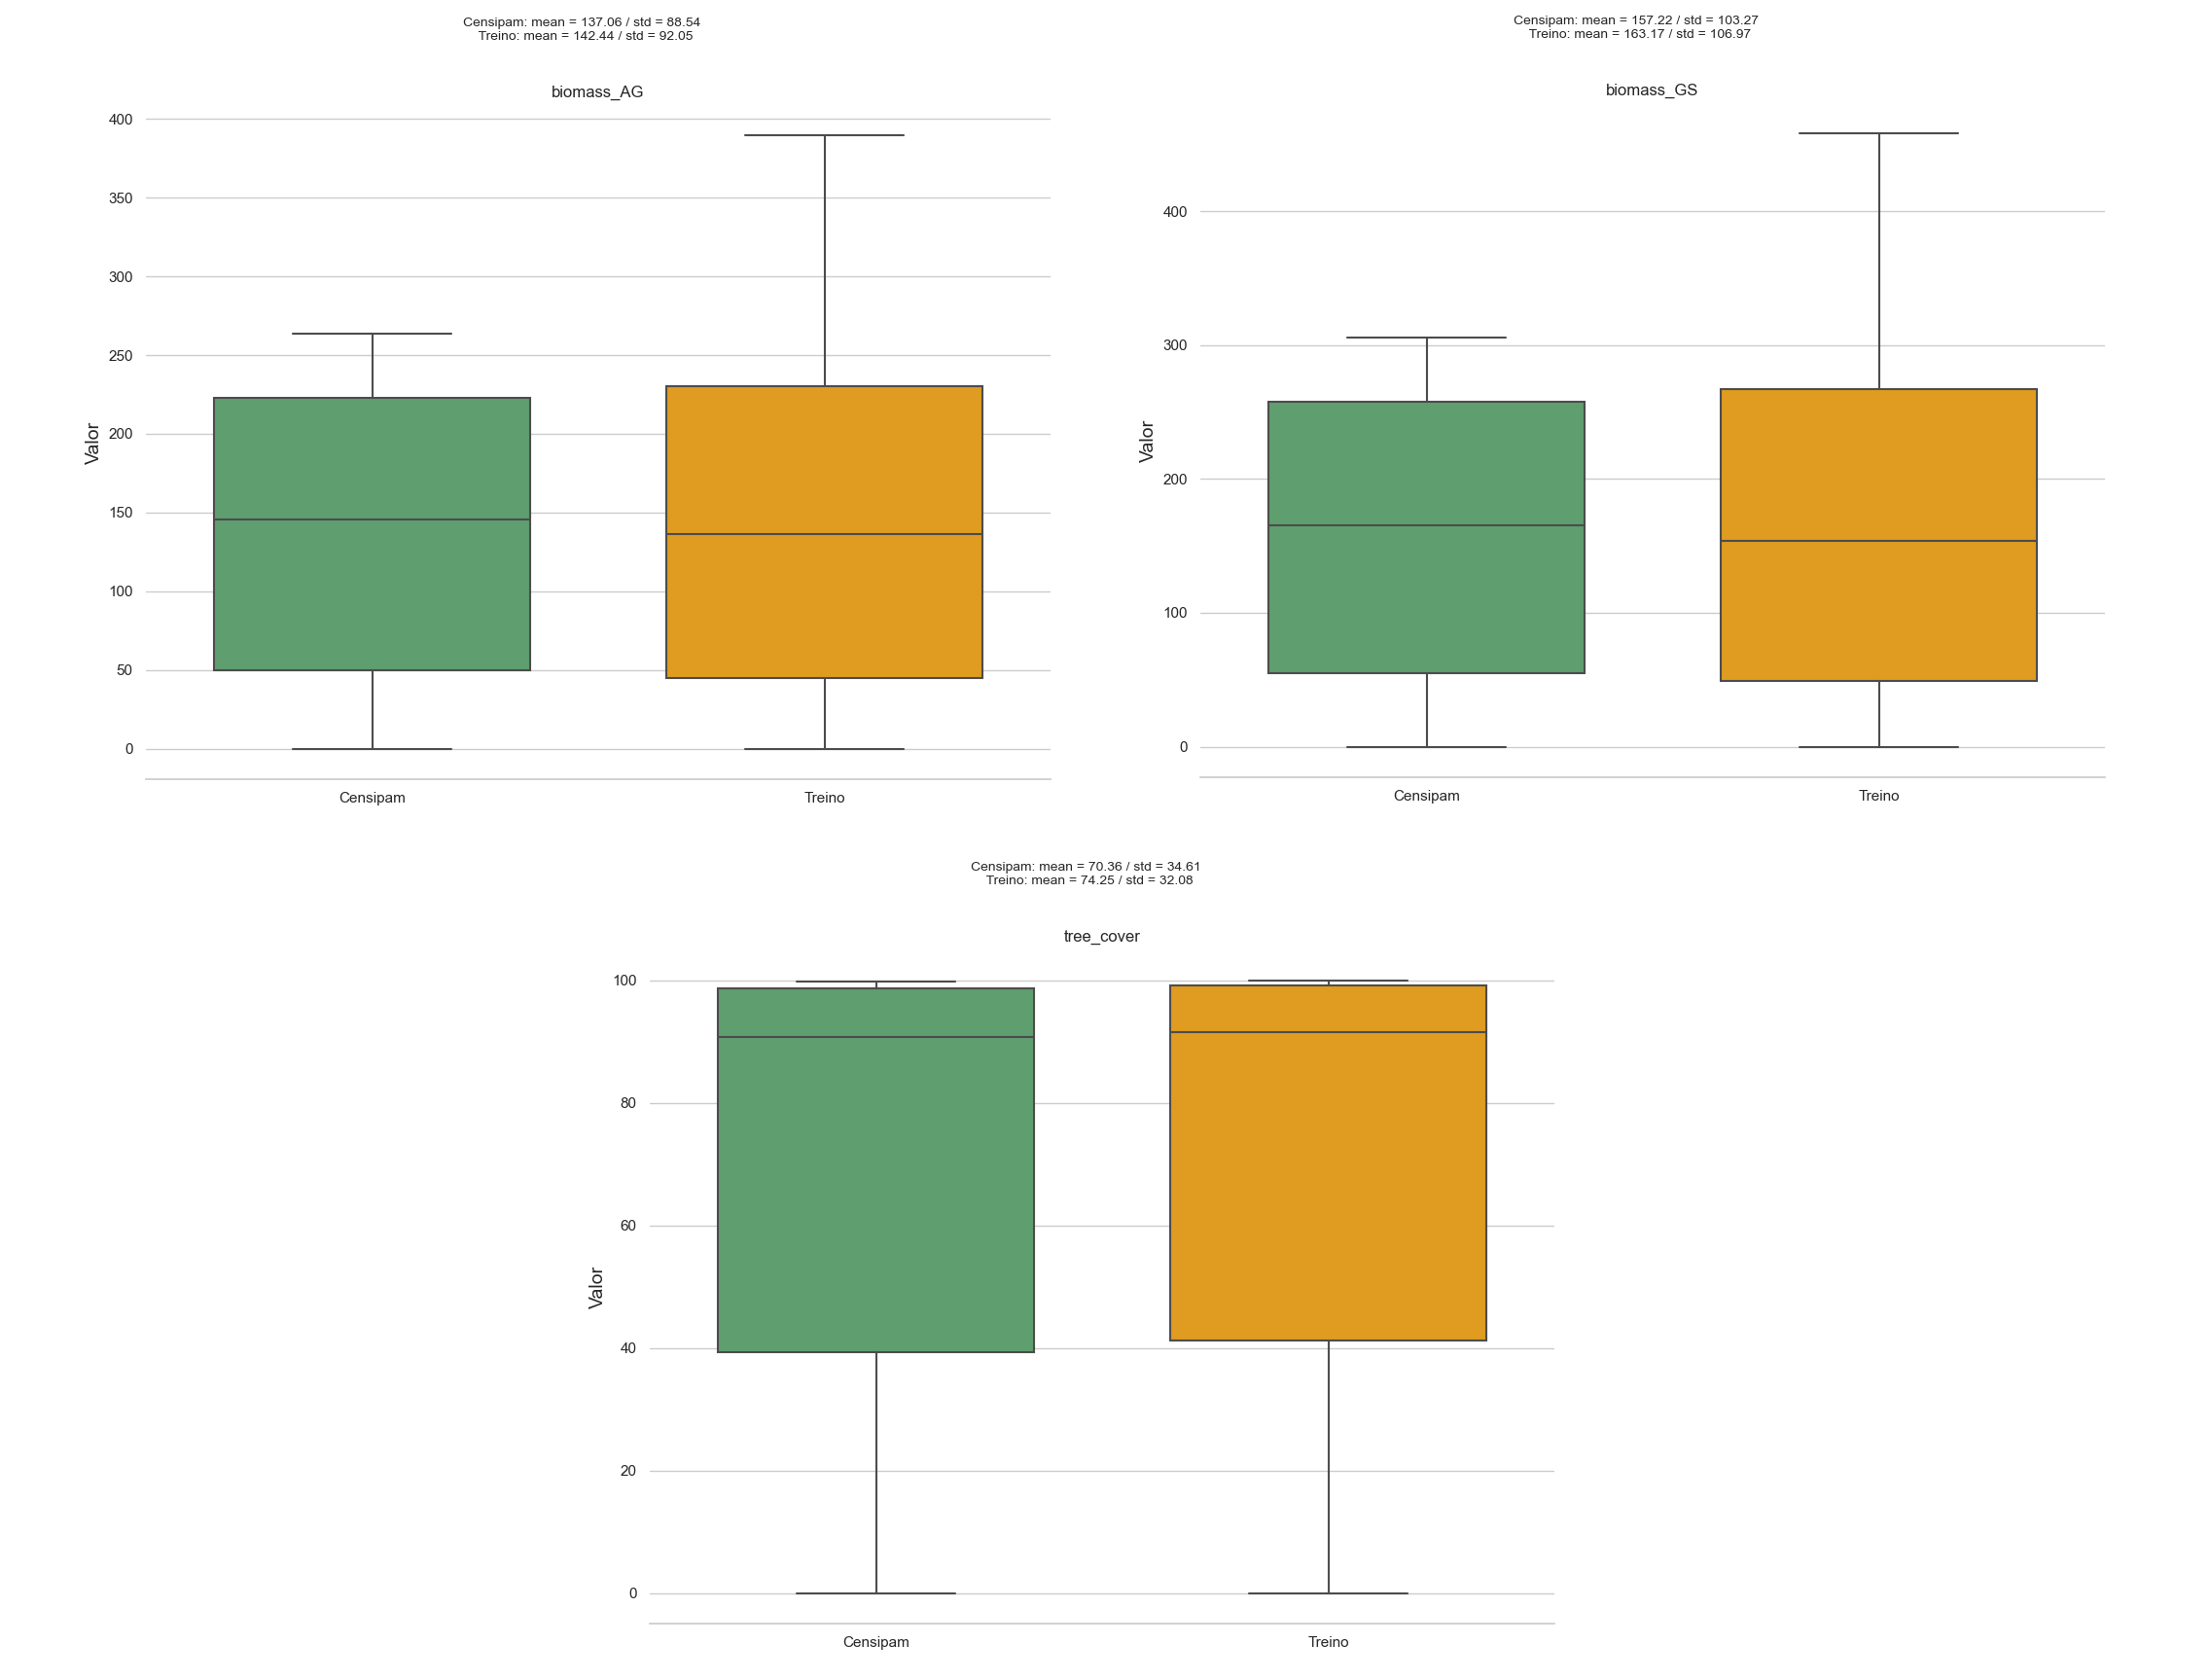
\includegraphics[scale=0.5]{tg1/figuras/graficosbons.png}
		\caption{Diagramas de Caixa de dados semelhantes}
            \label{fig:dadosbons}
	\end{minipage}
\end{figure}

A imagem \ref{fig:dadosbons} contém gráficos de caixa além de média e desvio padrão de algumas \textit{features} cujo as distribuições mostraram-se bastante similares entre os dois datasets. Estes dados possuem distribuições semelhantes, com valores de média e desvio padrão próximos indicando que ambos os dataset se assemelham em relação a estes dados.

No entanto, a diferença entre dados é significativa para vários outros dados. Na imagem \ref{fig:area} encontra-se o gráfico de caixa da \textit{feature} relativa a variação da área do incêndio. A diferença de escala entre as duas medidas é óbvia e indica que há algo de errado nestes dados. Este problema se revela em todos os dados relativos a área.

A escala sugere que talvez os dados estejam em unidades de medida diferentes, uma é metros quadrados e a outra em quilômetros quadrados. A imagem \ref{fig:corrigido} contém o mesmo gráfico, porém com os dados do servidor ajustados de quilômetro quadrado para metro quadrado. Como a semelhança entre os dados é alta, a hipótese de que trata-se de uma diferença de escala utilizada na geração dos dados é provavelmente verdadeira.

\begin{figure}[H]
	\centering
	\begin{minipage}{0.98\linewidth}
		\centering
		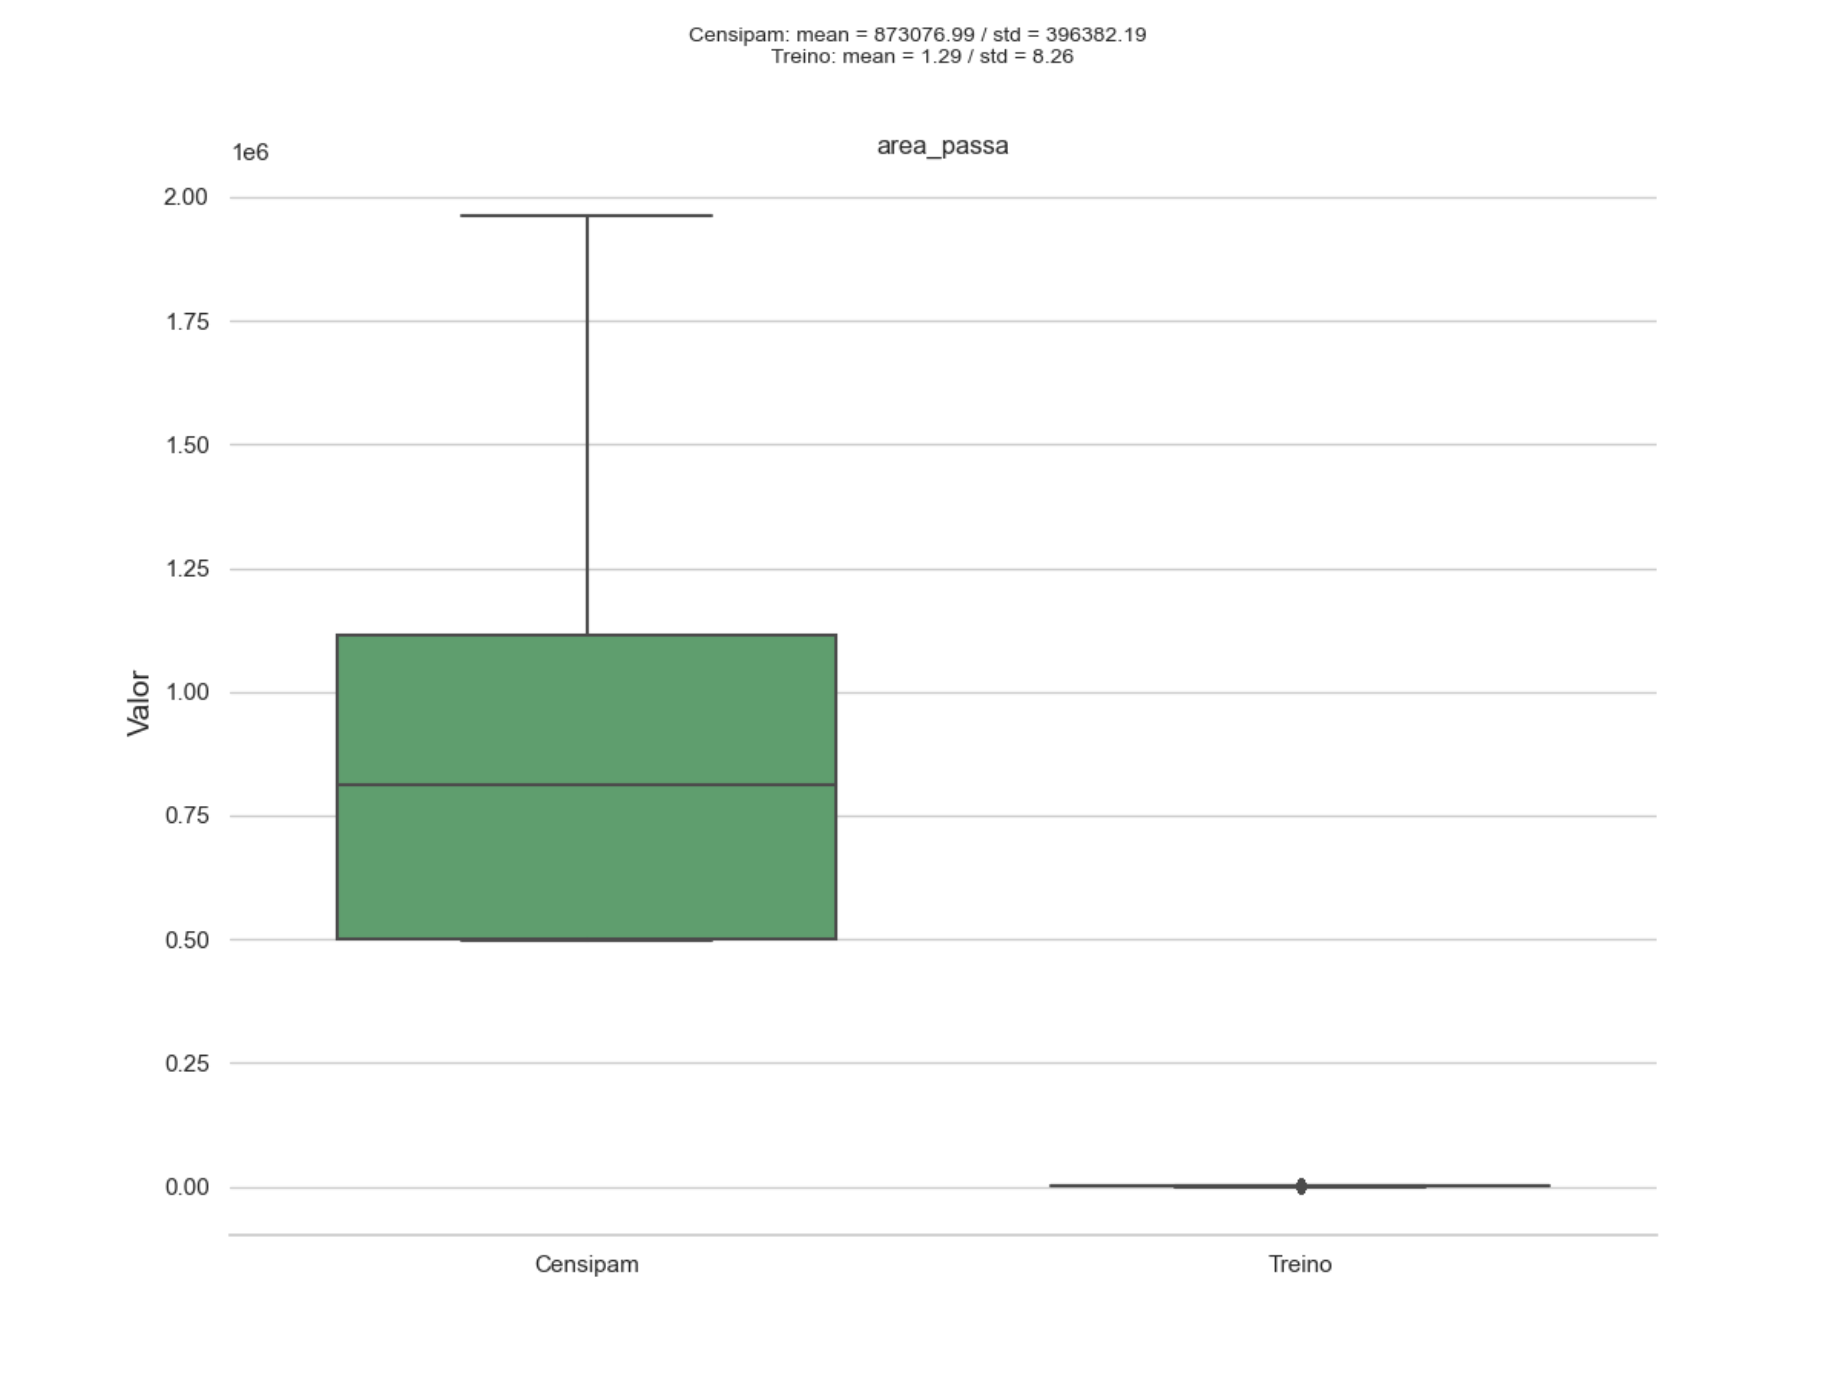
\includegraphics[scale=0.6]{tg1/figuras/area2.png}
		\caption{Diagramas de Caixa de variação de área da queimada}
            \label{fig:area}
	\end{minipage}
\end{figure}


\begin{figure}[H]
	\centering
	\begin{minipage}{0.98\linewidth}
		\centering
		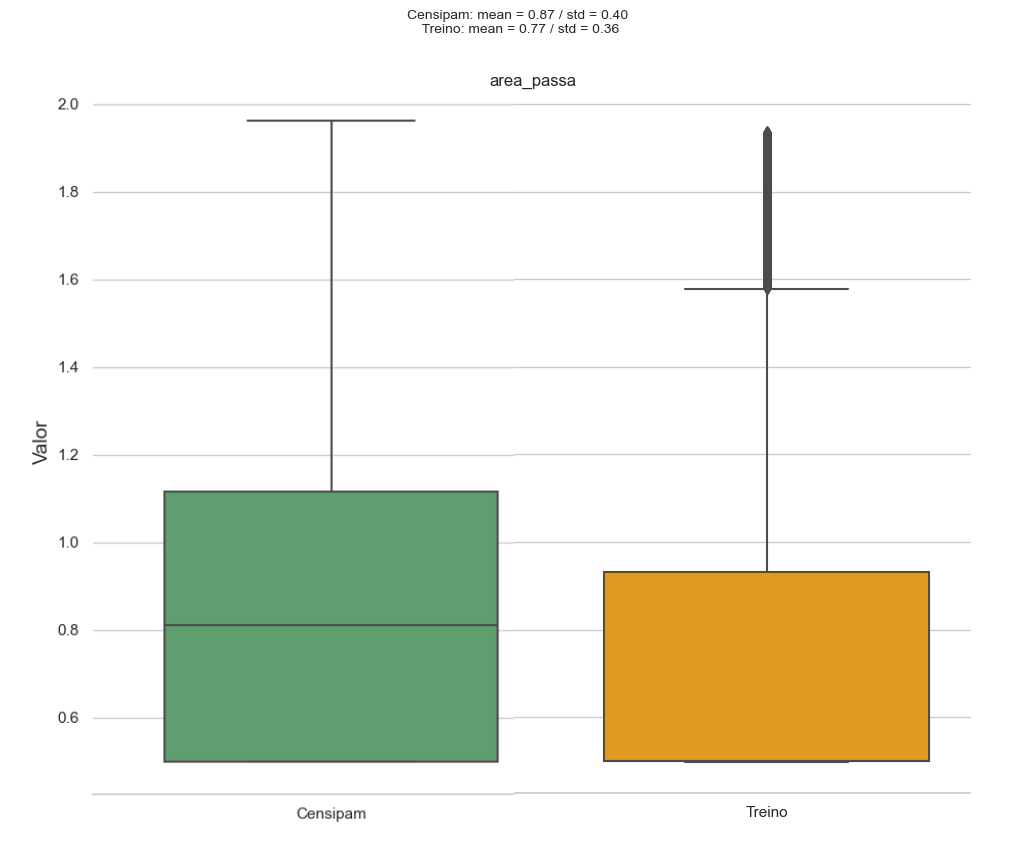
\includegraphics[scale=0.6]{tg1/figuras/corrigido.png}
		\caption{Diagramas de Caixa de variação de área da queimada corrigido em 10e6}
            \label{fig:corrigido}
	\end{minipage}
\end{figure}

Além disto, a \textit{features} geradas costumam apresentar problemas em geral, com todos os dados sendo aproximadamente zero, indicando algum problema com o algoritmo que as gera. Como este erro não surgiu durante o processo de gerar dados para o treinamento, nem ao se gerarem os dados em produção para o trabalho de \cite{BrunoScholess2023}. A hipótese mais provável é de que há alguma diferença nestes dados disponíveis no servidor do Censipam para o projeto atual que não foi levada em consideração durante o desenvolvimento do algoritmo. A inconsistência específica não foi encontrada.

Dessa forma, espera-se que o modelo não performe bem em produção, visto que não está recebendo dados adequados. Até o momento não tem como se verificar sua verdadeira performace visto que os dados novos do servidor não foram rotulados manualmente pelo pessoal do Censipam.





% \section{Evolução do modelo MLP}

% DROP OUT, NORM BATCH, LAYERS, BATCH SIZE, TREINAMENTO, MAQUINA UTILIZADA, ETC

% \section{Análise de Resultados}

% Na última etapa de calculo da precisão do modelo Random Forest, foi obtido os valores da tabela \ref{tab:rf} para quando classificamos o \textit{dataframe} de validação.

% \begin{table}[H]
% \caption{Precisão do modelo Random Forest}
% \label{tab:rf}
% \begin{tabular}{lllll}

%                  & Precision & Recall & F1-score & Quantidade \\
% 0                & 1.00      & 1.00   & 1.00     & 124125  \\
% 1                & 1.00      & 1.00   & 1.00     & 29652   \\
% 2                & 0.84      & 0.73   & 0.78     & 1866    \\
% 3                & 0.86      & 0.92   & 0.89     & 3615    \\
% Acurácia         &           &        & 0.99     & 159258  \\
% Média aritmética & 0.92      & 0.91   & 0.92     & 159258  \\
% Média ponderada  & 0.99      & 0.99   & 0.99     & 159258 
% \end{tabular}
% \end{table}


% A partir do resultado salvo em arquivo .csv, também é possível criarmos uma matriz de confusão para visualizarmos o comportamento da rede, conforme temos na figura \ref{fig:mcrf}. Quantos valores de cada tipo de fogo ela foi capaz de prever corretamente, e quantos ela errou, e para quais valores.

% \begin{figure}[htb]
% 	\centering
% 	\begin{minipage}{0.98\linewidth}
% 		\centering
% 		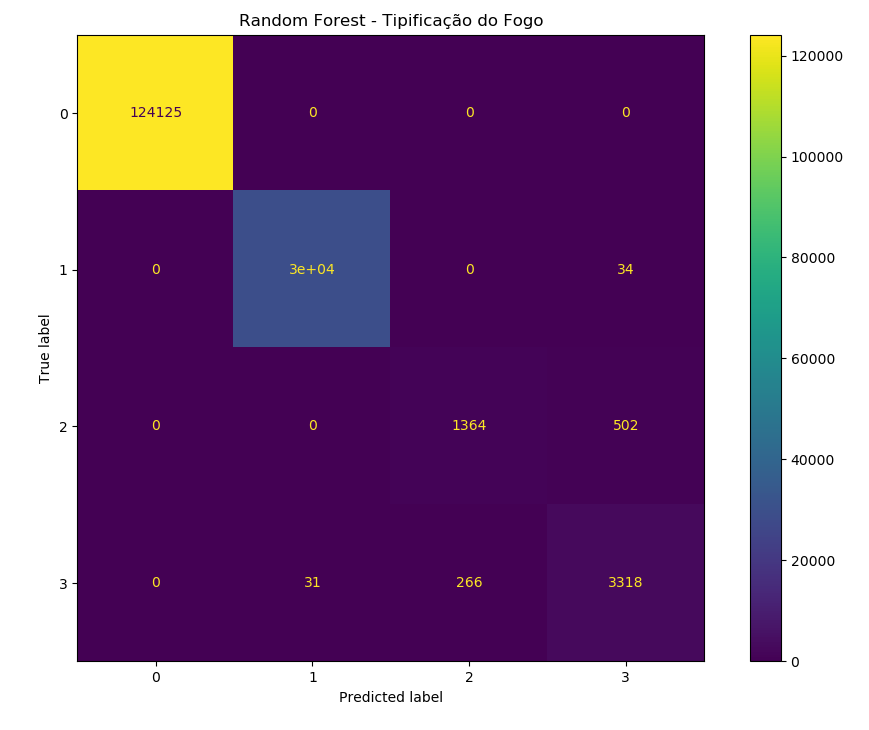
\includegraphics[width=\linewidth]{tg1/figuras/matrizconfusaorandomforest.png}
% 		\caption{Matriz de confusão para Random Forest} \label{fig:mcrf}
% 	\end{minipage}
% \end{figure}

% %\todo{COLOCAR METRICAS DO MLP}

% \begin{table}[H]
% \caption{Precisão do modelo MLP}
% \label{tab:rf}
% \begin{tabular}{lllll}

%                  & Precision & Recall & F1-score & Quantidade \\
% 0                & 1.00      & 1.00   & 1.00     & 124125  \\
% 1                & 0.98      & 1.00   & 0.99     & 29652   \\
% 2                & 0.69      & 0.66   & 0.68     & 1866    \\
% 3                & 0.79      & 0.84   & 0.81     & 3615    \\
% Acurácia         &           &        & ??     & 159258  \\
% Média aritmética & ??      & ??   & ??     & 159258  \\
% Média ponderada  & 0.99      & 0.99   & 0.99     & 159258 
% \end{tabular}
% \end{table}


\chapter{Conclusão}
\label{conclusao}

O trabalho apresentado teve como objetivo o desenvolvimento de um sistema de classificação de queimadas no território da Amazônia Legal, por meio de um algoritmo de inteligência artificial para séries temporais. Ademais, também foi-se desenvolvido com o propósito de eventualmente ser integrado ao sistema do Painel do Fogo do CENSIPAM.

A revisão literária indicou que embora este tipo de abordagem não seja inovadora no ramo do sensoriamento remoto em geral, é inovador no âmbito do sensoriamento dentro do território da Amazônia Legal.

O algoritmo desenvolvido é capaz de puxar dados oficiais e complementá-los, além de ser capaz de classificá-los com uma taxa de acurácia satisfatória.

Para trabalhos futuros, reserva-se a possibilidade de testar diferentes arquiteturas de redes neurais para séries temporais, como outras redes recorrentes ou redes convolucionais. Além disso, espera-se integrar o programa ao sistema oficial do CENSIPAM como uma ferramenta classificadora de seus dados, podendo assim, serem utilizados por autoridades competentes no combate à incêndios florestais.






% ------------------------------------------------------------------------
% ELEMENTOS PÓS-TEXTUAIS
% ------------------------------------------------------------------------
\postextual
% ------------------------------------------------------------------------

% ---
% Referências bibliográficas
% ---
% Seleciona o arquivo de estilo de citações
\IfStrEq*{\languagename}{english}{
\bibliographystyle{abntex2eng-alf}
}{
\bibliographystyle{abntex2-alf}
}
% Arquivos com as referências bibliográficas
\bibliography{tg1/referencias,tg1/references}

% ---
% Apêndices
% ---

\begin{apendicesenv}

% Imprime uma página indicando o início dos apêndices
\partapendices

% ----------------------------------------------------------
\chapter{Citações}
% ----------------------------------------------------------

Este modelo usa Bib\TeX\ para configurar as referências. Os arquivo referencias.bib e references.bib contêm várias entradas de bibliografia como modelos \cite{article,book,booklet,inbook}. Esses modelos podem ser utilizados para incluir outras entradas e citá-las por meio do seguinte comando:
\begin{verbatim}
\cite{nome_da_entrada}
\end{verbatim}

Por exemplo , a entrada
%\verbatimfont{\small}
\begin{verbatim}
@article{greenwade93,
    author  = "George D. Greenwade",
    title   = "The {C}omprehensive {T}ex {A}rchive {N}etwork ({CTAN})",
    year    = "1993",
    journal = "TUGBoat",
    volume  = "14",
    number  = "3",
    pages   = "342--351"
}
\end{verbatim}
%\verbatimfont{\normalfont}
pode ser citada no texto com
\begin{verbatim}
\cite{greenwade93}
\end{verbatim}
e a citação apareceria assim: \cite{greenwade93}.

Para fazer uma citação direta no formato ABNT, criamos o ambiente \verb|citacao|, que é uma simples generalização do ambiente \verb|quotation| (habilitado por padrão) com um campo específico de autor. Veja o exemplo a seguir:
\begin{verbatim}
\begin{citacao}{Carl Sagan}
    Alegações extraordinárias exigem evidências extraordinárias.
\end{citacao}
\end{verbatim}
Esse código gera uma citação assim:
\begin{citacao}{Carl Sagan}
    Alegações extraordinárias exigem evidências extraordinárias.
\end{citacao}
O comando \verb|\cite{...}| pode ser usado como indicação do autor:
\begin{verbatim}
\begin{citacao}{\cite{greenwade93}}
TEX is a typesetting program designed for high-quality composition of material
that contains a lot of mathematical and technical expressions. It has been 
adopted by many authors and publishers who generate technical books and papers. 
It was created by Professor Donald E. Knuth of Stanford University, originally 
for preparation of his book series ``The Art of Computer Programming''. TEX 
has been made freely available by Knuth.
\end{citacao}
\end{verbatim}
Naturalmente, a referência \verb|grennwade93| deve estar definida no arquivo Bib\TeX\ (aqui, \verb|references.bib|). Confira o resultado:
\begin{citacao}{\cite{greenwade93}}
TEX is a typesetting program designed for high-quality composition of material that contains a lot of mathematical and technical expressions. It has been adopted by many authors and publishers who generate technical books and papers. It was created by Professor Donald E. Knuth of Stanford University, originally for preparation of his book series ``The Art of Computer Programming''. TEX has been made freely available by Knuth.
\end{citacao}

%% ----------------------------------------------------------
\chapter{Códigos de programação}\label{apd:cdg}
% ----------------------------------------------------------

\section{Projeto do Controlador com Realimentação de Estados}
\lstinputlisting[language=Matlab,caption=Código de Matlab]{unbtex-example/codigos/controle.m}

\section{Exemplo de teste em Malha Fechada com Rampa}
\lstinputlisting[language=Python,caption=Código de Python]{unbtex-example/codigos/controleSmithPredictor.py}

\section{Redução modal}
\lstinputlisting[language=Julia,caption=Código de Julia]{unbtex-example/codigos/ModalReduction.jl}

\end{apendicesenv}
% ---

% ---
% Anexos
% ---

\begin{anexosenv}

% Imprime uma página indicando o início dos anexos
\partanexos

% ----------------------------------------------------------
\chapter{Figuras de exemplo}
% ----------------------------------------------------------

% Fonte: https://tex.stackexchange.com/a/231741/91816 (Gonzalo Medina)

\noindent\includegraphics[width=3cm]{example-image-a}\qquad
\includegraphics[width=3cm]{example-image-golden}\qquad
\includegraphics[width=3cm]{example-grid-100x100pt}

\noindent\includegraphics[height=5cm]{example-image-b} 

\noindent\includegraphics[scale=0.5]{example-image-c} 

\noindent\includegraphics[width=3cm]{example-image} 

% ----------------------------------------------------------
\chapter{Logo LaTeX}
% ----------------------------------------------------------

\vfill

\begin{center}
{\fontsize{50pt}{800pt}\selectfont \LaTeX}\
\end{center}

\vfill

\begin{center}
{\color{azulunb}\fontsize{50pt}{800pt}\selectfont \LaTeX}\
\end{center}

\vfill

\begin{center}
{\color{verdeunb}\fontsize{50pt}{800pt}\selectfont \LaTeX}\
\end{center}

\vfill

\end{anexosenv}

\end{document}